\subsection{UDP measurements}\label{sec_udp_mes}

\subsection*{Purpose:}

The purpose is to determine the maximum frequency that can be used in our system with the UDP protocol. To do so, we will measure the delay between to received packets and jitter and look at those values as a function of the delay used in the sending loop.

\subsection*{Test equipment:}

The sbRIO 9636 is connected to a computer running Ubuntu 14.04 LTS via an Ethernet cable of 1 gpbs. The computer runs the ROS nodes that are used for the project, thus it communicates with both the Geomagic Touch and the sbRIO. The sbRIO as well runs the entire code of the project.

\subsection*{Procedure:}

\begin{enumerate}
	\item The sbRIO is started and connected to the computer.
	\item The ROS node is started.
	\item Wireshark is started.% using this command: $tshark -i 1 -f udp -a duration:20 -w ~/wireshark_capture$
	\item Once the Wireshark recording is done the ROS node is stopped.
	\item The log files are retrieved to be analyzed using Matlab and Wireshark.
\end{enumerate}
Those steps are repeated for both the serial and parallel case for the following settings: 10 ms, 2 ms and 1 ms.


\subsection*{Measuring data:}

\begin{center}
  $\begin{tabular}{|c|c|c|c|c|}
    \hline
    \text{Frequency (Hz)} & \text{delay (ms)} & \text{Jitter ($\mu$s)} & \text{Packet loss (\%)}\\
    \hline
    99 & 10.1 & 4.66E-2 & 0 \\
    \hline
    474 & 2.1 & 5.51E-2 & 0.2 \\
    \hline
    638 & 1.6 & 1.16E-2 & 1.2 \\
    \hline
  \end{tabular}$
	\captionof{table}{Measurements of the UDP performances}
\end{center}
% \begin{figure}[H]
% 	\centering
% 	% This file was created by matlab2tikz.
%
%The latest updates can be retrieved from
%  http://www.mathworks.com/matlabcentral/fileexchange/22022-matlab2tikz-matlab2tikz
%where you can also make suggestions and rate matlab2tikz.
%
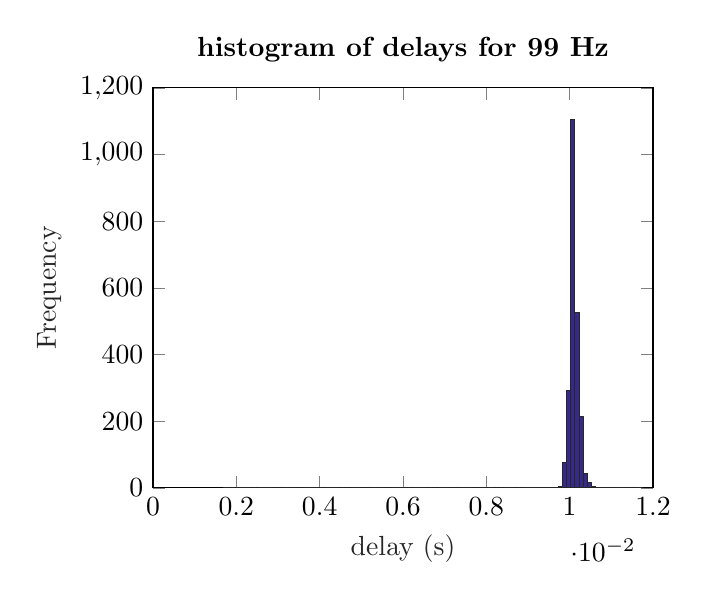
\begin{tikzpicture}

\begin{axis}[%
width=2.5in,
height=2in,
scale only axis,
point meta min=1,
point meta max=2,
colormap={mymap}{[1pt] rgb(0pt)=(0.2081,0.1663,0.5292); rgb(1pt)=(0.211624,0.189781,0.577676); rgb(2pt)=(0.212252,0.213771,0.626971); rgb(3pt)=(0.2081,0.2386,0.677086); rgb(4pt)=(0.195905,0.264457,0.7279); rgb(5pt)=(0.170729,0.291938,0.779248); rgb(6pt)=(0.125271,0.324243,0.830271); rgb(7pt)=(0.0591333,0.359833,0.868333); rgb(8pt)=(0.0116952,0.38751,0.881957); rgb(9pt)=(0.00595714,0.408614,0.882843); rgb(10pt)=(0.0165143,0.4266,0.878633); rgb(11pt)=(0.0328524,0.443043,0.871957); rgb(12pt)=(0.0498143,0.458571,0.864057); rgb(13pt)=(0.0629333,0.47369,0.855438); rgb(14pt)=(0.0722667,0.488667,0.8467); rgb(15pt)=(0.0779429,0.503986,0.838371); rgb(16pt)=(0.0793476,0.520024,0.831181); rgb(17pt)=(0.0749429,0.537543,0.826271); rgb(18pt)=(0.0640571,0.556986,0.823957); rgb(19pt)=(0.0487714,0.577224,0.822829); rgb(20pt)=(0.0343429,0.596581,0.819852); rgb(21pt)=(0.0265,0.6137,0.8135); rgb(22pt)=(0.0238905,0.628662,0.803762); rgb(23pt)=(0.0230905,0.641786,0.791267); rgb(24pt)=(0.0227714,0.653486,0.776757); rgb(25pt)=(0.0266619,0.664195,0.760719); rgb(26pt)=(0.0383714,0.674271,0.743552); rgb(27pt)=(0.0589714,0.683757,0.725386); rgb(28pt)=(0.0843,0.692833,0.706167); rgb(29pt)=(0.113295,0.7015,0.685857); rgb(30pt)=(0.145271,0.709757,0.664629); rgb(31pt)=(0.180133,0.717657,0.642433); rgb(32pt)=(0.217829,0.725043,0.619262); rgb(33pt)=(0.258643,0.731714,0.595429); rgb(34pt)=(0.302171,0.737605,0.571186); rgb(35pt)=(0.348167,0.742433,0.547267); rgb(36pt)=(0.395257,0.7459,0.524443); rgb(37pt)=(0.44201,0.748081,0.503314); rgb(38pt)=(0.487124,0.749062,0.483976); rgb(39pt)=(0.530029,0.749114,0.466114); rgb(40pt)=(0.570857,0.748519,0.44939); rgb(41pt)=(0.609852,0.747314,0.433686); rgb(42pt)=(0.6473,0.7456,0.4188); rgb(43pt)=(0.683419,0.743476,0.404433); rgb(44pt)=(0.71841,0.741133,0.390476); rgb(45pt)=(0.752486,0.7384,0.376814); rgb(46pt)=(0.785843,0.735567,0.363271); rgb(47pt)=(0.818505,0.732733,0.34979); rgb(48pt)=(0.850657,0.7299,0.336029); rgb(49pt)=(0.882433,0.727433,0.3217); rgb(50pt)=(0.913933,0.725786,0.306276); rgb(51pt)=(0.944957,0.726114,0.288643); rgb(52pt)=(0.973895,0.731395,0.266648); rgb(53pt)=(0.993771,0.745457,0.240348); rgb(54pt)=(0.999043,0.765314,0.216414); rgb(55pt)=(0.995533,0.786057,0.196652); rgb(56pt)=(0.988,0.8066,0.179367); rgb(57pt)=(0.978857,0.827143,0.163314); rgb(58pt)=(0.9697,0.848138,0.147452); rgb(59pt)=(0.962586,0.870514,0.1309); rgb(60pt)=(0.958871,0.8949,0.113243); rgb(61pt)=(0.959824,0.921833,0.0948381); rgb(62pt)=(0.9661,0.951443,0.0755333); rgb(63pt)=(0.9763,0.9831,0.0538)},
xmin=0,
xmax=0.012,
xlabel style={font=\color{white!15!black}},
xlabel={delay (s)},
ymin=0,
ymax=1200,
ylabel style={font=\color{white!15!black}},
ylabel={Frequency},
axis background/.style={fill=white},
title style={font=\bfseries},
title={histogram of delays for 99 Hz}
]

\addplot[area legend, table/row sep=crcr, patch, patch type=rectangle, shader=flat corner, draw=white!15!black, forget plot, patch table with point meta={%
1	2	3	4	1\\
6	7	8	9	1\\
11	12	13	14	1\\
16	17	18	19	1\\
21	22	23	24	1\\
26	27	28	29	1\\
31	32	33	34	1\\
36	37	38	39	1\\
41	42	43	44	1\\
46	47	48	49	1\\
51	52	53	54	1\\
56	57	58	59	1\\
61	62	63	64	1\\
66	67	68	69	1\\
71	72	73	74	1\\
76	77	78	79	1\\
81	82	83	84	1\\
86	87	88	89	1\\
91	92	93	94	1\\
96	97	98	99	1\\
101	102	103	104	1\\
106	107	108	109	1\\
111	112	113	114	1\\
116	117	118	119	1\\
121	122	123	124	1\\
126	127	128	129	1\\
131	132	133	134	1\\
136	137	138	139	1\\
141	142	143	144	1\\
146	147	148	149	1\\
151	152	153	154	1\\
156	157	158	159	1\\
161	162	163	164	1\\
166	167	168	169	1\\
171	172	173	174	1\\
176	177	178	179	1\\
181	182	183	184	1\\
186	187	188	189	1\\
191	192	193	194	1\\
196	197	198	199	1\\
201	202	203	204	1\\
206	207	208	209	1\\
211	212	213	214	1\\
216	217	218	219	1\\
221	222	223	224	1\\
226	227	228	229	1\\
231	232	233	234	1\\
236	237	238	239	1\\
241	242	243	244	1\\
246	247	248	249	1\\
251	252	253	254	1\\
256	257	258	259	1\\
261	262	263	264	1\\
266	267	268	269	1\\
271	272	273	274	1\\
276	277	278	279	1\\
281	282	283	284	1\\
286	287	288	289	1\\
291	292	293	294	1\\
296	297	298	299	1\\
301	302	303	304	1\\
306	307	308	309	1\\
311	312	313	314	1\\
316	317	318	319	1\\
321	322	323	324	1\\
326	327	328	329	1\\
331	332	333	334	1\\
336	337	338	339	1\\
341	342	343	344	1\\
346	347	348	349	1\\
351	352	353	354	1\\
356	357	358	359	1\\
361	362	363	364	1\\
366	367	368	369	1\\
371	372	373	374	1\\
376	377	378	379	1\\
381	382	383	384	1\\
386	387	388	389	1\\
391	392	393	394	1\\
396	397	398	399	1\\
401	402	403	404	1\\
406	407	408	409	1\\
411	412	413	414	1\\
416	417	418	419	1\\
421	422	423	424	1\\
426	427	428	429	1\\
431	432	433	434	1\\
436	437	438	439	1\\
441	442	443	444	1\\
446	447	448	449	1\\
451	452	453	454	1\\
456	457	458	459	1\\
461	462	463	464	1\\
466	467	468	469	1\\
471	472	473	474	1\\
476	477	478	479	1\\
481	482	483	484	1\\
486	487	488	489	1\\
491	492	493	494	1\\
496	497	498	499	1\\
}]
table[row sep=crcr] {%
x	y\\
0.001682	0\\
0.001682	0\\
0.001682	1\\
0.00178253	1\\
0.00178253	0\\
0.00178253	0\\
0.00178253	0\\
0.00178253	0\\
0.00188306	0\\
0.00188306	0\\
0.00188306	0\\
0.00188306	0\\
0.00188306	0\\
0.00198359	0\\
0.00198359	0\\
0.00198359	0\\
0.00198359	0\\
0.00198359	0\\
0.00208412	0\\
0.00208412	0\\
0.00208412	0\\
0.00208412	0\\
0.00208412	0\\
0.00218465	0\\
0.00218465	0\\
0.00218465	0\\
0.00218465	0\\
0.00218465	0\\
0.00228518	0\\
0.00228518	0\\
0.00228518	0\\
0.00228518	0\\
0.00228518	0\\
0.00238571	0\\
0.00238571	0\\
0.00238571	0\\
0.00238571	0\\
0.00238571	0\\
0.00248624	0\\
0.00248624	0\\
0.00248624	0\\
0.00248624	0\\
0.00248624	0\\
0.00258677	0\\
0.00258677	0\\
0.00258677	0\\
0.00258677	0\\
0.00258677	0\\
0.00268730000000001	0\\
0.00268730000000001	0\\
0.0026873	0\\
0.0026873	0\\
0.0026873	0\\
0.00278783000000001	0\\
0.00278783000000001	0\\
0.00278783000000001	0\\
0.00278783000000001	0\\
0.00278783000000001	0\\
0.00288836000000001	0\\
0.00288836000000001	0\\
0.00288836000000001	0\\
0.00288836000000001	0\\
0.00288836000000001	0\\
0.00298889000000001	0\\
0.00298889000000001	0\\
0.00298889000000001	0\\
0.00298889000000001	0\\
0.00298889000000001	0\\
0.00308942000000001	0\\
0.00308942000000001	0\\
0.00308942000000001	0\\
0.00308942000000001	0\\
0.00308942000000001	0\\
0.00318995000000001	0\\
0.00318995000000001	0\\
0.00318995000000001	0\\
0.00318995000000001	0\\
0.00318995000000001	0\\
0.00329048000000001	0\\
0.00329048000000001	0\\
0.00329048000000001	0\\
0.00329048000000001	0\\
0.00329048000000001	0\\
0.00339101000000001	0\\
0.00339101000000001	0\\
0.00339101000000001	0\\
0.00339101000000001	0\\
0.00339101000000001	0\\
0.00349154000000001	0\\
0.00349154000000001	0\\
0.00349154000000001	0\\
0.00349154000000001	0\\
0.00349154000000001	0\\
0.00359207000000001	0\\
0.00359207000000001	0\\
0.00359207000000001	0\\
0.00359207000000001	0\\
0.00359207000000001	0\\
0.00369260000000001	0\\
0.00369260000000001	0\\
0.00369260000000001	0\\
0.00369260000000001	0\\
0.00369260000000001	0\\
0.00379313000000001	0\\
0.00379313000000001	0\\
0.00379313000000001	0\\
0.00379313000000001	0\\
0.00379313000000001	0\\
0.00389366000000001	0\\
0.00389366000000001	0\\
0.00389366000000001	0\\
0.00389366000000001	0\\
0.00389366000000001	0\\
0.00399419000000001	0\\
0.00399419000000001	0\\
0.00399419000000001	0\\
0.00399419000000001	0\\
0.00399419000000001	0\\
0.00409472000000001	0\\
0.00409472000000001	0\\
0.00409472000000001	0\\
0.00409472000000001	0\\
0.00409472000000001	0\\
0.00419525000000001	0\\
0.00419525000000001	0\\
0.00419525000000001	0\\
0.00419525000000001	0\\
0.00419525000000001	0\\
0.00429578000000001	0\\
0.00429578000000001	0\\
0.00429578000000001	0\\
0.00429578000000001	0\\
0.00429578000000001	0\\
0.00439631000000001	0\\
0.00439631000000001	0\\
0.00439631000000001	0\\
0.00439631000000001	0\\
0.00439631000000001	0\\
0.00449684000000001	0\\
0.00449684000000001	0\\
0.00449684000000001	0\\
0.00449684000000001	0\\
0.00449684000000001	0\\
0.00459737000000002	0\\
0.00459737000000002	0\\
0.00459737000000001	0\\
0.00459737000000001	0\\
0.00459737000000001	0\\
0.00469790000000002	0\\
0.00469790000000002	0\\
0.00469790000000002	0\\
0.00469790000000002	0\\
0.00469790000000002	0\\
0.00479843000000002	0\\
0.00479843000000002	0\\
0.00479843000000002	0\\
0.00479843000000002	0\\
0.00479843000000002	0\\
0.00489896000000002	0\\
0.00489896000000002	0\\
0.00489896000000002	0\\
0.00489896000000002	0\\
0.00489896000000002	0\\
0.00499949000000002	0\\
0.00499949000000002	0\\
0.00499949000000002	0\\
0.00499949000000002	0\\
0.00499949000000002	0\\
0.00510002000000002	0\\
0.00510002000000002	0\\
0.00510002000000002	0\\
0.00510002000000002	0\\
0.00510002000000002	0\\
0.00520055000000002	0\\
0.00520055000000002	0\\
0.00520055000000002	0\\
0.00520055000000002	0\\
0.00520055000000002	0\\
0.00530108000000002	0\\
0.00530108000000002	0\\
0.00530108000000002	0\\
0.00530108000000002	0\\
0.00530108000000002	0\\
0.00540161000000002	0\\
0.00540161000000002	0\\
0.00540161000000002	0\\
0.00540161000000002	0\\
0.00540161000000002	0\\
0.00550214000000002	0\\
0.00550214000000002	0\\
0.00550214000000002	0\\
0.00550214000000002	0\\
0.00550214000000002	0\\
0.00560267000000002	0\\
0.00560267000000002	0\\
0.00560267000000002	0\\
0.00560267000000002	0\\
0.00560267000000002	0\\
0.00570320000000002	0\\
0.00570320000000002	0\\
0.00570320000000002	0\\
0.00570320000000002	0\\
0.00570320000000002	0\\
0.00580373000000002	0\\
0.00580373000000002	0\\
0.00580373000000002	0\\
0.00580373000000002	0\\
0.00580373000000002	0\\
0.00590426000000002	0\\
0.00590426000000002	0\\
0.00590426000000002	0\\
0.00590426000000002	0\\
0.00590426000000002	0\\
0.00600479000000002	0\\
0.00600479000000002	0\\
0.00600479000000002	0\\
0.00600479000000002	0\\
0.00600479000000002	0\\
0.00610532000000002	0\\
0.00610532000000002	0\\
0.00610532000000002	0\\
0.00610532000000002	0\\
0.00610532000000002	0\\
0.00620585000000002	0\\
0.00620585000000002	0\\
0.00620585000000002	0\\
0.00620585000000002	0\\
0.00620585000000002	0\\
0.00630638000000002	0\\
0.00630638000000002	0\\
0.00630638000000002	0\\
0.00630638000000002	0\\
0.00630638000000002	0\\
0.00640691000000002	0\\
0.00640691000000002	0\\
0.00640691000000003	0\\
0.00640691000000003	0\\
0.00640691000000003	0\\
0.00650744000000003	0\\
0.00650744000000003	0\\
0.00650744000000002	0\\
0.00650744000000002	0\\
0.00650744000000002	0\\
0.00660797000000003	0\\
0.00660797000000003	0\\
0.00660797000000003	0\\
0.00660797000000003	0\\
0.00660797000000003	0\\
0.00670850000000003	0\\
0.00670850000000003	0\\
0.00670850000000003	0\\
0.00670850000000003	0\\
0.00670850000000003	0\\
0.00680903000000003	0\\
0.00680903000000003	0\\
0.00680903000000003	0\\
0.00680903000000003	0\\
0.00680903000000003	0\\
0.00690956000000003	0\\
0.00690956000000003	0\\
0.00690956000000003	0\\
0.00690956000000003	0\\
0.00690956000000003	0\\
0.00701009000000003	0\\
0.00701009000000003	0\\
0.00701009000000003	0\\
0.00701009000000003	0\\
0.00701009000000003	0\\
0.00711062000000003	0\\
0.00711062000000003	0\\
0.00711062000000003	0\\
0.00711062000000003	0\\
0.00711062000000003	0\\
0.00721115000000003	0\\
0.00721115000000003	0\\
0.00721115000000003	0\\
0.00721115000000003	0\\
0.00721115000000003	0\\
0.00731168000000003	0\\
0.00731168000000003	0\\
0.00731168000000003	0\\
0.00731168000000003	0\\
0.00731168000000003	0\\
0.00741221000000003	0\\
0.00741221000000003	0\\
0.00741221000000003	0\\
0.00741221000000003	0\\
0.00741221000000003	0\\
0.00751274000000003	0\\
0.00751274000000003	0\\
0.00751274000000003	0\\
0.00751274000000003	0\\
0.00751274000000003	0\\
0.00761327000000003	0\\
0.00761327000000003	0\\
0.00761327000000003	0\\
0.00761327000000003	0\\
0.00761327000000003	0\\
0.00771380000000003	0\\
0.00771380000000003	0\\
0.00771380000000003	0\\
0.00771380000000003	0\\
0.00771380000000003	0\\
0.00781433000000003	0\\
0.00781433000000003	0\\
0.00781433000000003	0\\
0.00781433000000003	0\\
0.00781433000000003	0\\
0.00791486000000003	0\\
0.00791486000000003	0\\
0.00791486000000003	0\\
0.00791486000000003	0\\
0.00791486000000003	0\\
0.00801539000000003	0\\
0.00801539000000003	0\\
0.00801539000000003	0\\
0.00801539000000003	0\\
0.00801539000000003	0\\
0.00811592000000003	0\\
0.00811592000000003	0\\
0.00811592000000003	0\\
0.00811592000000003	0\\
0.00811592000000003	0\\
0.00821645000000003	0\\
0.00821645000000003	0\\
0.00821645000000003	0\\
0.00821645000000003	0\\
0.00821645000000003	0\\
0.00831698000000003	0\\
0.00831698000000003	0\\
0.00831698000000003	0\\
0.00831698000000003	0\\
0.00831698000000003	0\\
0.00841751000000003	0\\
0.00841751000000003	0\\
0.00841751000000003	0\\
0.00841751000000003	0\\
0.00841751000000003	0\\
0.00851804000000003	0\\
0.00851804000000003	0\\
0.00851804000000004	0\\
0.00851804000000004	0\\
0.00851804000000004	0\\
0.00861857000000004	0\\
0.00861857000000004	0\\
0.00861857000000004	0\\
0.00861857000000004	0\\
0.00861857000000004	0\\
0.00871910000000004	0\\
0.00871910000000004	0\\
0.00871910000000004	0\\
0.00871910000000004	0\\
0.00871910000000004	0\\
0.00881963000000003	0\\
0.00881963000000003	0\\
0.00881963000000004	0\\
0.00881963000000004	0\\
0.00881963000000004	0\\
0.00892016000000004	0\\
0.00892016000000004	0\\
0.00892016000000004	0\\
0.00892016000000004	0\\
0.00892016000000004	1\\
0.00902069000000004	1\\
0.00902069000000004	0\\
0.00902069000000004	0\\
0.00902069000000004	0\\
0.00902069000000004	1\\
0.00912122000000004	1\\
0.00912122000000004	0\\
0.00912122000000004	0\\
0.00912122000000004	0\\
0.00912122000000004	0\\
0.00922175000000004	0\\
0.00922175000000004	0\\
0.00922175000000004	0\\
0.00922175000000004	0\\
0.00922175000000004	1\\
0.00932228000000004	1\\
0.00932228000000004	0\\
0.00932228000000004	0\\
0.00932228000000004	0\\
0.00932228000000004	1\\
0.00942281000000004	1\\
0.00942281000000004	0\\
0.00942281000000004	0\\
0.00942281000000004	0\\
0.00942281000000004	0\\
0.00952334000000004	0\\
0.00952334000000004	0\\
0.00952334000000004	0\\
0.00952334000000004	0\\
0.00952334000000004	0\\
0.00962387000000004	0\\
0.00962387000000004	0\\
0.00962387000000004	0\\
0.00962387000000004	0\\
0.00962387000000004	0\\
0.00972440000000004	0\\
0.00972440000000004	0\\
0.00972440000000004	0\\
0.00972440000000004	0\\
0.00972440000000004	4\\
0.00982493000000004	4\\
0.00982493000000004	0\\
0.00982493000000004	0\\
0.00982493000000004	0\\
0.00982493000000004	75\\
0.00992546000000004	75\\
0.00992546000000004	0\\
0.00992546000000004	0\\
0.00992546000000004	0\\
0.00992546000000004	293\\
0.01002599	293\\
0.01002599	0\\
0.01002599	0\\
0.01002599	0\\
0.01002599	1106\\
0.01012652	1106\\
0.01012652	0\\
0.01012652	0\\
0.01012652	0\\
0.01012652	525\\
0.01022705	525\\
0.01022705	0\\
0.01022705	0\\
0.01022705	0\\
0.01022705	214\\
0.01032758	214\\
0.01032758	0\\
0.01032758	0\\
0.01032758	0\\
0.01032758	44\\
0.01042811	44\\
0.01042811	0\\
0.01042811	0\\
0.01042811	0\\
0.01042811	15\\
0.01052864	15\\
0.01052864	0\\
0.01052864	0\\
0.01052864	0\\
0.01052864	3\\
0.01062917	3\\
0.01062917	0\\
0.01062917	0\\
0.01062917	0\\
0.01062917	1\\
0.0107297	1\\
0.0107297	0\\
0.0107297	0\\
0.0107297	0\\
0.0107297	1\\
0.01083023	1\\
0.01083023	0\\
0.01083023	0\\
0.01083023	0\\
0.01083023	0\\
0.01093076	0\\
0.01093076	0\\
0.01093076	0\\
0.01093076	0\\
0.01093076	1\\
0.01103129	1\\
0.01103129	0\\
0.01103129	0\\
0.01103129	0\\
0.01103129	0\\
0.01113182	0\\
0.01113182	0\\
0.01113182	0\\
0.01113182	0\\
0.01113182	1\\
0.01123235	1\\
0.01123235	0\\
0.01123235	0\\
0.01123235	0\\
0.01123235	2\\
0.01133288	2\\
0.01133288	0\\
0.01133288	0\\
0.01133288	0\\
0.01133288	0\\
0.01143341	0\\
0.01143341	0\\
0.0114334100000001	0\\
0.0114334100000001	0\\
0.0114334100000001	0\\
0.01153394	0\\
0.01153394	0\\
0.01153394	0\\
0.01153394	0\\
0.01153394	0\\
0.01163447	0\\
0.01163447	0\\
0.0116344700000001	0\\
0.0116344700000001	0\\
0.0116344700000001	1\\
0.0117350000000001	1\\
0.0117350000000001	0\\
0.0117350000000001	0\\
};
\end{axis}
\end{tikzpicture}%
% 	\caption{10ms}
% \end{figure} 
% \begin{figure}[H]
% 		\centering
% 	    % This file was created by matlab2tikz.
%
%The latest updates can be retrieved from
%  http://www.mathworks.com/matlabcentral/fileexchange/22022-matlab2tikz-matlab2tikz
%where you can also make suggestions and rate matlab2tikz.
%
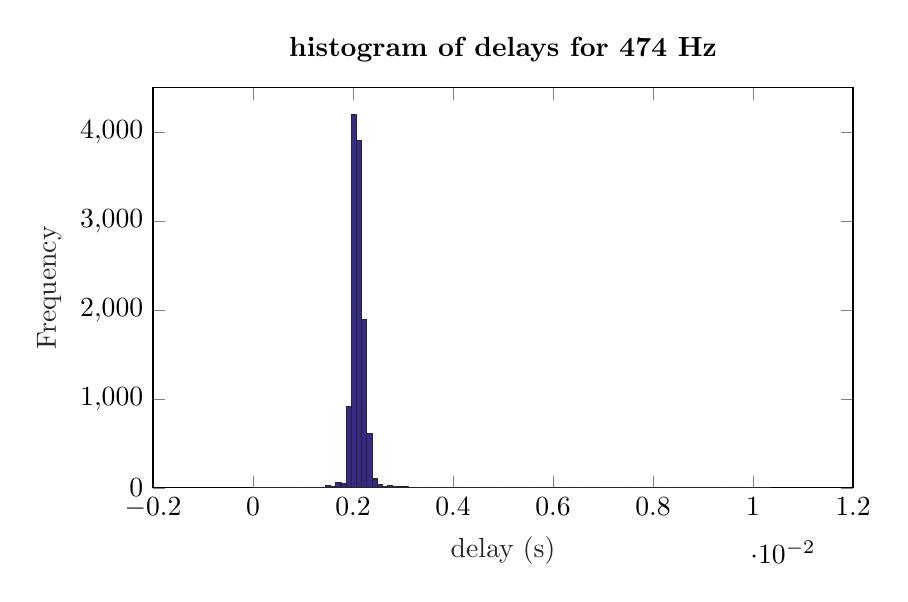
\begin{tikzpicture}

\begin{axis}[%
width=3.5in,
height=2in,
scale only axis,
point meta min=1,
point meta max=2,
colormap={mymap}{[1pt] rgb(0pt)=(0.2081,0.1663,0.5292); rgb(1pt)=(0.211624,0.189781,0.577676); rgb(2pt)=(0.212252,0.213771,0.626971); rgb(3pt)=(0.2081,0.2386,0.677086); rgb(4pt)=(0.195905,0.264457,0.7279); rgb(5pt)=(0.170729,0.291938,0.779248); rgb(6pt)=(0.125271,0.324243,0.830271); rgb(7pt)=(0.0591333,0.359833,0.868333); rgb(8pt)=(0.0116952,0.38751,0.881957); rgb(9pt)=(0.00595714,0.408614,0.882843); rgb(10pt)=(0.0165143,0.4266,0.878633); rgb(11pt)=(0.0328524,0.443043,0.871957); rgb(12pt)=(0.0498143,0.458571,0.864057); rgb(13pt)=(0.0629333,0.47369,0.855438); rgb(14pt)=(0.0722667,0.488667,0.8467); rgb(15pt)=(0.0779429,0.503986,0.838371); rgb(16pt)=(0.0793476,0.520024,0.831181); rgb(17pt)=(0.0749429,0.537543,0.826271); rgb(18pt)=(0.0640571,0.556986,0.823957); rgb(19pt)=(0.0487714,0.577224,0.822829); rgb(20pt)=(0.0343429,0.596581,0.819852); rgb(21pt)=(0.0265,0.6137,0.8135); rgb(22pt)=(0.0238905,0.628662,0.803762); rgb(23pt)=(0.0230905,0.641786,0.791267); rgb(24pt)=(0.0227714,0.653486,0.776757); rgb(25pt)=(0.0266619,0.664195,0.760719); rgb(26pt)=(0.0383714,0.674271,0.743552); rgb(27pt)=(0.0589714,0.683757,0.725386); rgb(28pt)=(0.0843,0.692833,0.706167); rgb(29pt)=(0.113295,0.7015,0.685857); rgb(30pt)=(0.145271,0.709757,0.664629); rgb(31pt)=(0.180133,0.717657,0.642433); rgb(32pt)=(0.217829,0.725043,0.619262); rgb(33pt)=(0.258643,0.731714,0.595429); rgb(34pt)=(0.302171,0.737605,0.571186); rgb(35pt)=(0.348167,0.742433,0.547267); rgb(36pt)=(0.395257,0.7459,0.524443); rgb(37pt)=(0.44201,0.748081,0.503314); rgb(38pt)=(0.487124,0.749062,0.483976); rgb(39pt)=(0.530029,0.749114,0.466114); rgb(40pt)=(0.570857,0.748519,0.44939); rgb(41pt)=(0.609852,0.747314,0.433686); rgb(42pt)=(0.6473,0.7456,0.4188); rgb(43pt)=(0.683419,0.743476,0.404433); rgb(44pt)=(0.71841,0.741133,0.390476); rgb(45pt)=(0.752486,0.7384,0.376814); rgb(46pt)=(0.785843,0.735567,0.363271); rgb(47pt)=(0.818505,0.732733,0.34979); rgb(48pt)=(0.850657,0.7299,0.336029); rgb(49pt)=(0.882433,0.727433,0.3217); rgb(50pt)=(0.913933,0.725786,0.306276); rgb(51pt)=(0.944957,0.726114,0.288643); rgb(52pt)=(0.973895,0.731395,0.266648); rgb(53pt)=(0.993771,0.745457,0.240348); rgb(54pt)=(0.999043,0.765314,0.216414); rgb(55pt)=(0.995533,0.786057,0.196652); rgb(56pt)=(0.988,0.8066,0.179367); rgb(57pt)=(0.978857,0.827143,0.163314); rgb(58pt)=(0.9697,0.848138,0.147452); rgb(59pt)=(0.962586,0.870514,0.1309); rgb(60pt)=(0.958871,0.8949,0.113243); rgb(61pt)=(0.959824,0.921833,0.0948381); rgb(62pt)=(0.9661,0.951443,0.0755333); rgb(63pt)=(0.9763,0.9831,0.0538)},
xmin=-0.002,
xmax=0.012,
xlabel style={font=\color{white!15!black}},
xlabel={delay (s)},
ymin=0,
ymax=4500,
ylabel style={font=\color{white!15!black}},
ylabel={Frequency},
axis background/.style={fill=white},
title style={font=\bfseries},
title={histogram of delays for 474 Hz}
]

\addplot[area legend, table/row sep=crcr, patch, patch type=rectangle, shader=flat corner, draw=white!15!black, forget plot, patch table with point meta={%
1	2	3	4	1\\
6	7	8	9	1\\
11	12	13	14	1\\
16	17	18	19	1\\
21	22	23	24	1\\
26	27	28	29	1\\
31	32	33	34	1\\
36	37	38	39	1\\
41	42	43	44	1\\
46	47	48	49	1\\
51	52	53	54	1\\
56	57	58	59	1\\
61	62	63	64	1\\
66	67	68	69	1\\
71	72	73	74	1\\
76	77	78	79	1\\
81	82	83	84	1\\
86	87	88	89	1\\
91	92	93	94	1\\
96	97	98	99	1\\
101	102	103	104	1\\
106	107	108	109	1\\
111	112	113	114	1\\
116	117	118	119	1\\
121	122	123	124	1\\
126	127	128	129	1\\
131	132	133	134	1\\
136	137	138	139	1\\
141	142	143	144	1\\
146	147	148	149	1\\
151	152	153	154	1\\
156	157	158	159	1\\
161	162	163	164	1\\
166	167	168	169	1\\
171	172	173	174	1\\
176	177	178	179	1\\
181	182	183	184	1\\
186	187	188	189	1\\
191	192	193	194	1\\
196	197	198	199	1\\
201	202	203	204	1\\
206	207	208	209	1\\
211	212	213	214	1\\
216	217	218	219	1\\
221	222	223	224	1\\
226	227	228	229	1\\
231	232	233	234	1\\
236	237	238	239	1\\
241	242	243	244	1\\
246	247	248	249	1\\
251	252	253	254	1\\
256	257	258	259	1\\
261	262	263	264	1\\
266	267	268	269	1\\
271	272	273	274	1\\
276	277	278	279	1\\
281	282	283	284	1\\
286	287	288	289	1\\
291	292	293	294	1\\
296	297	298	299	1\\
301	302	303	304	1\\
306	307	308	309	1\\
311	312	313	314	1\\
316	317	318	319	1\\
321	322	323	324	1\\
326	327	328	329	1\\
331	332	333	334	1\\
336	337	338	339	1\\
341	342	343	344	1\\
346	347	348	349	1\\
351	352	353	354	1\\
356	357	358	359	1\\
361	362	363	364	1\\
366	367	368	369	1\\
371	372	373	374	1\\
376	377	378	379	1\\
381	382	383	384	1\\
386	387	388	389	1\\
391	392	393	394	1\\
396	397	398	399	1\\
401	402	403	404	1\\
406	407	408	409	1\\
411	412	413	414	1\\
416	417	418	419	1\\
421	422	423	424	1\\
426	427	428	429	1\\
431	432	433	434	1\\
436	437	438	439	1\\
441	442	443	444	1\\
446	447	448	449	1\\
451	452	453	454	1\\
456	457	458	459	1\\
461	462	463	464	1\\
466	467	468	469	1\\
471	472	473	474	1\\
476	477	478	479	1\\
481	482	483	484	1\\
486	487	488	489	1\\
491	492	493	494	1\\
496	497	498	499	1\\
}]
table[row sep=crcr] {%
x	y\\
-6.7762635780344e-21	0\\
-6.7762635780344e-21	0\\
-6.7762635780344e-21	1\\
0.000103580000000001	1\\
0.000103580000000001	0\\
0.000103580000000001	0\\
0.000103580000000001	0\\
0.000103580000000001	0\\
0.000207160000000002	0\\
0.000207160000000002	0\\
0.000207160000000002	0\\
0.000207160000000002	0\\
0.000207160000000002	0\\
0.000310740000000003	0\\
0.000310740000000003	0\\
0.000310740000000003	0\\
0.000310740000000003	0\\
0.000310740000000003	0\\
0.000414320000000004	0\\
0.000414320000000004	0\\
0.000414320000000004	0\\
0.000414320000000004	0\\
0.000414320000000004	0\\
0.000517900000000005	0\\
0.000517900000000005	0\\
0.000517900000000005	0\\
0.000517900000000005	0\\
0.000517900000000005	0\\
0.000621480000000005	0\\
0.000621480000000005	0\\
0.000621480000000005	0\\
0.000621480000000005	0\\
0.000621480000000005	0\\
0.000725060000000006	0\\
0.000725060000000006	0\\
0.000725060000000006	0\\
0.000725060000000006	0\\
0.000725060000000006	0\\
0.000828640000000007	0\\
0.000828640000000007	0\\
0.000828640000000007	0\\
0.000828640000000007	0\\
0.000828640000000007	0\\
0.000932220000000008	0\\
0.000932220000000008	0\\
0.000932220000000008	0\\
0.000932220000000008	0\\
0.000932220000000008	0\\
0.00103580000000001	0\\
0.00103580000000001	0\\
0.00103580000000001	0\\
0.00103580000000001	0\\
0.00103580000000001	0\\
0.00113938000000001	0\\
0.00113938000000001	0\\
0.00113938000000001	0\\
0.00113938000000001	0\\
0.00113938000000001	0\\
0.00124296000000001	0\\
0.00124296000000001	0\\
0.00124296000000001	0\\
0.00124296000000001	0\\
0.00124296000000001	0\\
0.00134654000000001	0\\
0.00134654000000001	0\\
0.00134654000000001	0\\
0.00134654000000001	0\\
0.00134654000000001	9\\
0.00145012000000001	9\\
0.00145012000000001	0\\
0.00145012000000001	0\\
0.00145012000000001	0\\
0.00145012000000001	28\\
0.00155370000000001	28\\
0.00155370000000001	0\\
0.00155370000000001	0\\
0.00155370000000001	0\\
0.00155370000000001	18\\
0.00165728000000001	18\\
0.00165728000000001	0\\
0.00165728000000001	0\\
0.00165728000000001	0\\
0.00165728000000001	56\\
0.00176086000000001	56\\
0.00176086000000001	0\\
0.00176086000000002	0\\
0.00176086000000002	0\\
0.00176086000000002	45\\
0.00186444000000002	45\\
0.00186444000000002	0\\
0.00186444000000002	0\\
0.00186444000000002	0\\
0.00186444000000002	916\\
0.00196802000000002	916\\
0.00196802000000002	0\\
0.00196802000000002	0\\
0.00196802000000002	0\\
0.00196802000000002	4199\\
0.00207160000000002	4199\\
0.00207160000000002	0\\
0.00207160000000002	0\\
0.00207160000000002	0\\
0.00207160000000002	3910\\
0.00217518000000002	3910\\
0.00217518000000002	0\\
0.00217518000000002	0\\
0.00217518000000002	0\\
0.00217518000000002	1896\\
0.00227876000000002	1896\\
0.00227876000000002	0\\
0.00227876000000002	0\\
0.00227876000000002	0\\
0.00227876000000002	608\\
0.00238234000000002	608\\
0.00238234000000002	0\\
0.00238234000000002	0\\
0.00238234000000002	0\\
0.00238234000000002	100\\
0.00248592000000002	100\\
0.00248592000000002	0\\
0.00248592000000002	0\\
0.00248592000000002	0\\
0.00248592000000002	37\\
0.00258950000000002	37\\
0.00258950000000002	0\\
0.00258950000000002	0\\
0.00258950000000002	0\\
0.00258950000000002	15\\
0.00269308000000002	15\\
0.00269308000000002	0\\
0.00269308000000002	0\\
0.00269308000000002	0\\
0.00269308000000002	22\\
0.00279666000000002	22\\
0.00279666000000002	0\\
0.00279666000000002	0\\
0.00279666000000002	0\\
0.00279666000000002	10\\
0.00290024000000003	10\\
0.00290024000000003	0\\
0.00290024000000002	0\\
0.00290024000000002	0\\
0.00290024000000002	12\\
0.00300382000000003	12\\
0.00300382000000003	0\\
0.00300382000000003	0\\
0.00300382000000003	0\\
0.00300382000000003	10\\
0.00310740000000003	10\\
0.00310740000000003	0\\
0.00310740000000003	0\\
0.00310740000000003	0\\
0.00310740000000003	8\\
0.00321098000000003	8\\
0.00321098000000003	0\\
0.00321098000000003	0\\
0.00321098000000003	0\\
0.00321098000000003	3\\
0.00331456000000003	3\\
0.00331456000000003	0\\
0.00331456000000003	0\\
0.00331456000000003	0\\
0.00331456000000003	2\\
0.00341814000000003	2\\
0.00341814000000003	0\\
0.00341814000000003	0\\
0.00341814000000003	0\\
0.00341814000000003	2\\
0.00352172000000003	2\\
0.00352172000000003	0\\
0.00352172000000003	0\\
0.00352172000000003	0\\
0.00352172000000003	1\\
0.00362530000000003	1\\
0.00362530000000003	0\\
0.00362530000000003	0\\
0.00362530000000003	0\\
0.00362530000000003	3\\
0.00372888000000003	3\\
0.00372888000000003	0\\
0.00372888000000003	0\\
0.00372888000000003	0\\
0.00372888000000003	1\\
0.00383246000000003	1\\
0.00383246000000003	0\\
0.00383246000000003	0\\
0.00383246000000003	0\\
0.00383246000000003	3\\
0.00393604000000003	3\\
0.00393604000000003	0\\
0.00393604000000003	0\\
0.00393604000000003	0\\
0.00393604000000003	2\\
0.00403962000000003	2\\
0.00403962000000003	0\\
0.00403962000000003	0\\
0.00403962000000003	0\\
0.00403962000000003	1\\
0.00414320000000004	1\\
0.00414320000000004	0\\
0.00414320000000004	0\\
0.00414320000000004	0\\
0.00414320000000004	3\\
0.00424678000000004	3\\
0.00424678000000004	0\\
0.00424678000000004	0\\
0.00424678000000004	0\\
0.00424678000000004	1\\
0.00435036000000004	1\\
0.00435036000000004	0\\
0.00435036000000004	0\\
0.00435036000000004	0\\
0.00435036000000004	0\\
0.00445394000000004	0\\
0.00445394000000004	0\\
0.00445394000000004	0\\
0.00445394000000004	0\\
0.00445394000000004	0\\
0.00455752000000004	0\\
0.00455752000000004	0\\
0.00455752000000004	0\\
0.00455752000000004	0\\
0.00455752000000004	0\\
0.00466110000000004	0\\
0.00466110000000004	0\\
0.00466110000000004	0\\
0.00466110000000004	0\\
0.00466110000000004	0\\
0.00476468000000004	0\\
0.00476468000000004	0\\
0.00476468000000004	0\\
0.00476468000000004	0\\
0.00476468000000004	0\\
0.00486826000000004	0\\
0.00486826000000004	0\\
0.00486826000000004	0\\
0.00486826000000004	0\\
0.00486826000000004	1\\
0.00497184000000004	1\\
0.00497184000000004	0\\
0.00497184000000004	0\\
0.00497184000000004	0\\
0.00497184000000004	0\\
0.00507542000000004	0\\
0.00507542000000004	0\\
0.00507542000000004	0\\
0.00507542000000004	0\\
0.00507542000000004	1\\
0.00517900000000004	1\\
0.00517900000000004	0\\
0.00517900000000004	0\\
0.00517900000000004	0\\
0.00517900000000004	0\\
0.00528258000000005	0\\
0.00528258000000005	0\\
0.00528258000000005	0\\
0.00528258000000005	0\\
0.00528258000000005	0\\
0.00538616000000005	0\\
0.00538616000000005	0\\
0.00538616000000005	0\\
0.00538616000000005	0\\
0.00538616000000005	0\\
0.00548974000000005	0\\
0.00548974000000005	0\\
0.00548974000000005	0\\
0.00548974000000005	0\\
0.00548974000000005	0\\
0.00559332000000005	0\\
0.00559332000000005	0\\
0.00559332000000005	0\\
0.00559332000000005	0\\
0.00559332000000005	1\\
0.00569690000000005	1\\
0.00569690000000005	0\\
0.00569690000000005	0\\
0.00569690000000005	0\\
0.00569690000000005	2\\
0.00580048000000005	2\\
0.00580048000000005	0\\
0.00580048000000005	0\\
0.00580048000000005	0\\
0.00580048000000005	1\\
0.00590406000000005	1\\
0.00590406000000005	0\\
0.00590406000000005	0\\
0.00590406000000005	0\\
0.00590406000000005	1\\
0.00600764000000005	1\\
0.00600764000000005	0\\
0.00600764000000005	0\\
0.00600764000000005	0\\
0.00600764000000005	0\\
0.00611122000000005	0\\
0.00611122000000005	0\\
0.00611122000000005	0\\
0.00611122000000005	0\\
0.00611122000000005	0\\
0.00621480000000005	0\\
0.00621480000000005	0\\
0.00621480000000005	0\\
0.00621480000000005	0\\
0.00621480000000005	0\\
0.00631838000000005	0\\
0.00631838000000005	0\\
0.00631838000000005	0\\
0.00631838000000005	0\\
0.00631838000000005	0\\
0.00642196000000006	0\\
0.00642196000000006	0\\
0.00642196000000006	0\\
0.00642196000000006	0\\
0.00642196000000006	0\\
0.00652554000000006	0\\
0.00652554000000006	0\\
0.00652554000000006	0\\
0.00652554000000006	0\\
0.00652554000000006	1\\
0.00662912000000006	1\\
0.00662912000000006	0\\
0.00662912000000006	0\\
0.00662912000000006	0\\
0.00662912000000006	0\\
0.00673270000000006	0\\
0.00673270000000006	0\\
0.00673270000000006	0\\
0.00673270000000006	0\\
0.00673270000000006	0\\
0.00683628000000006	0\\
0.00683628000000006	0\\
0.00683628000000006	0\\
0.00683628000000006	0\\
0.00683628000000006	0\\
0.00693986000000006	0\\
0.00693986000000006	0\\
0.00693986000000006	0\\
0.00693986000000006	0\\
0.00693986000000006	0\\
0.00704344000000006	0\\
0.00704344000000006	0\\
0.00704344000000006	0\\
0.00704344000000006	0\\
0.00704344000000006	1\\
0.00714702000000006	1\\
0.00714702000000006	0\\
0.00714702000000006	0\\
0.00714702000000006	0\\
0.00714702000000006	0\\
0.00725060000000006	0\\
0.00725060000000006	0\\
0.00725060000000006	0\\
0.00725060000000006	0\\
0.00725060000000006	1\\
0.00735418000000006	1\\
0.00735418000000006	0\\
0.00735418000000006	0\\
0.00735418000000006	0\\
0.00735418000000006	0\\
0.00745776000000006	0\\
0.00745776000000006	0\\
0.00745776000000006	0\\
0.00745776000000006	0\\
0.00745776000000006	0\\
0.00756134000000006	0\\
0.00756134000000006	0\\
0.00756134000000007	0\\
0.00756134000000007	0\\
0.00756134000000007	0\\
0.00766492000000007	0\\
0.00766492000000007	0\\
0.00766492000000007	0\\
0.00766492000000007	0\\
0.00766492000000007	0\\
0.00776850000000007	0\\
0.00776850000000007	0\\
0.00776850000000007	0\\
0.00776850000000007	0\\
0.00776850000000007	0\\
0.00787208000000007	0\\
0.00787208000000007	0\\
0.00787208000000007	0\\
0.00787208000000007	0\\
0.00787208000000007	1\\
0.00797566000000007	1\\
0.00797566000000007	0\\
0.00797566000000007	0\\
0.00797566000000007	0\\
0.00797566000000007	0\\
0.00807924000000007	0\\
0.00807924000000007	0\\
0.00807924000000007	0\\
0.00807924000000007	0\\
0.00807924000000007	0\\
0.00818282000000007	0\\
0.00818282000000007	0\\
0.00818282000000007	0\\
0.00818282000000007	0\\
0.00818282000000007	0\\
0.00828640000000007	0\\
0.00828640000000007	0\\
0.00828640000000007	0\\
0.00828640000000007	0\\
0.00828640000000007	0\\
0.00838998000000007	0\\
0.00838998000000007	0\\
0.00838998000000007	0\\
0.00838998000000007	0\\
0.00838998000000007	0\\
0.00849356000000007	0\\
0.00849356000000007	0\\
0.00849356000000007	0\\
0.00849356000000007	0\\
0.00849356000000007	0\\
0.00859714000000007	0\\
0.00859714000000007	0\\
0.00859714000000007	0\\
0.00859714000000007	0\\
0.00859714000000007	0\\
0.00870072000000007	0\\
0.00870072000000007	0\\
0.00870072000000007	0\\
0.00870072000000007	0\\
0.00870072000000007	0\\
0.00880430000000008	0\\
0.00880430000000008	0\\
0.00880430000000008	0\\
0.00880430000000008	0\\
0.00880430000000008	0\\
0.00890788000000008	0\\
0.00890788000000008	0\\
0.00890788000000008	0\\
0.00890788000000008	0\\
0.00890788000000008	0\\
0.00901146000000008	0\\
0.00901146000000008	0\\
0.00901146000000008	0\\
0.00901146000000008	0\\
0.00901146000000008	0\\
0.00911504000000008	0\\
0.00911504000000008	0\\
0.00911504000000008	0\\
0.00911504000000008	0\\
0.00911504000000008	0\\
0.00921862000000008	0\\
0.00921862000000008	0\\
0.00921862000000008	0\\
0.00921862000000008	0\\
0.00921862000000008	0\\
0.00932220000000008	0\\
0.00932220000000008	0\\
0.00932220000000008	0\\
0.00932220000000008	0\\
0.00932220000000008	0\\
0.00942578000000008	0\\
0.00942578000000008	0\\
0.00942578000000008	0\\
0.00942578000000008	0\\
0.00942578000000008	0\\
0.00952936000000008	0\\
0.00952936000000008	0\\
0.00952936000000008	0\\
0.00952936000000008	0\\
0.00952936000000008	0\\
0.00963294000000008	0\\
0.00963294000000008	0\\
0.00963294000000008	0\\
0.00963294000000008	0\\
0.00963294000000008	0\\
0.00973652000000008	0\\
0.00973652000000008	0\\
0.00973652000000008	0\\
0.00973652000000008	0\\
0.00973652000000008	0\\
0.00984010000000008	0\\
0.00984010000000008	0\\
0.00984010000000008	0\\
0.00984010000000008	0\\
0.00984010000000008	0\\
0.00994368000000008	0\\
0.00994368000000008	0\\
0.00994368000000009	0\\
0.00994368000000009	0\\
0.00994368000000009	1\\
0.0100472600000001	1\\
0.0100472600000001	0\\
0.0100472600000001	0\\
0.0100472600000001	0\\
0.0100472600000001	1\\
0.0101508400000001	1\\
0.0101508400000001	0\\
0.0101508400000001	0\\
0.0101508400000001	0\\
0.0101508400000001	0\\
0.0102544200000001	0\\
0.0102544200000001	0\\
0.0102544200000001	0\\
0.0102544200000001	0\\
0.0102544200000001	1\\
0.0103580000000001	1\\
0.0103580000000001	0\\
0.0103580000000001	0\\
};
\end{axis}
\end{tikzpicture}%
% 	    \caption{2ms}
% \end{figure} 
% \begin{figure}[H]
% 	    \centering
% 	    % This file was created by matlab2tikz.
%
%The latest updates can be retrieved from
%  http://www.mathworks.com/matlabcentral/fileexchange/22022-matlab2tikz-matlab2tikz
%where you can also make suggestions and rate matlab2tikz.
%
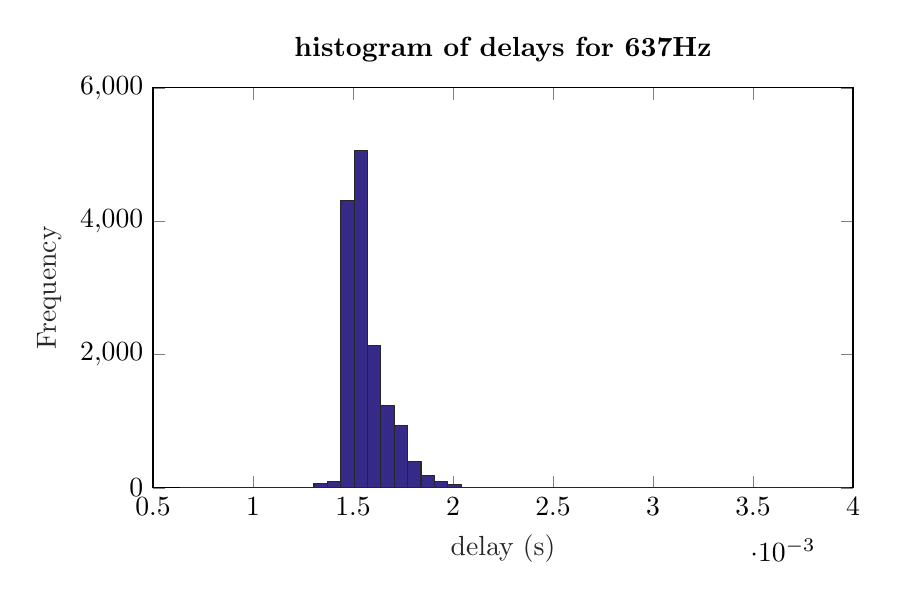
\begin{tikzpicture}

\begin{axis}[%
width=3.5in,
height=2in,
at={(1.255in,1.115in)},
scale only axis,
point meta min=1,
point meta max=2,
colormap={mymap}{[1pt] rgb(0pt)=(0.2081,0.1663,0.5292); rgb(1pt)=(0.211624,0.189781,0.577676); rgb(2pt)=(0.212252,0.213771,0.626971); rgb(3pt)=(0.2081,0.2386,0.677086); rgb(4pt)=(0.195905,0.264457,0.7279); rgb(5pt)=(0.170729,0.291938,0.779248); rgb(6pt)=(0.125271,0.324243,0.830271); rgb(7pt)=(0.0591333,0.359833,0.868333); rgb(8pt)=(0.0116952,0.38751,0.881957); rgb(9pt)=(0.00595714,0.408614,0.882843); rgb(10pt)=(0.0165143,0.4266,0.878633); rgb(11pt)=(0.0328524,0.443043,0.871957); rgb(12pt)=(0.0498143,0.458571,0.864057); rgb(13pt)=(0.0629333,0.47369,0.855438); rgb(14pt)=(0.0722667,0.488667,0.8467); rgb(15pt)=(0.0779429,0.503986,0.838371); rgb(16pt)=(0.0793476,0.520024,0.831181); rgb(17pt)=(0.0749429,0.537543,0.826271); rgb(18pt)=(0.0640571,0.556986,0.823957); rgb(19pt)=(0.0487714,0.577224,0.822829); rgb(20pt)=(0.0343429,0.596581,0.819852); rgb(21pt)=(0.0265,0.6137,0.8135); rgb(22pt)=(0.0238905,0.628662,0.803762); rgb(23pt)=(0.0230905,0.641786,0.791267); rgb(24pt)=(0.0227714,0.653486,0.776757); rgb(25pt)=(0.0266619,0.664195,0.760719); rgb(26pt)=(0.0383714,0.674271,0.743552); rgb(27pt)=(0.0589714,0.683757,0.725386); rgb(28pt)=(0.0843,0.692833,0.706167); rgb(29pt)=(0.113295,0.7015,0.685857); rgb(30pt)=(0.145271,0.709757,0.664629); rgb(31pt)=(0.180133,0.717657,0.642433); rgb(32pt)=(0.217829,0.725043,0.619262); rgb(33pt)=(0.258643,0.731714,0.595429); rgb(34pt)=(0.302171,0.737605,0.571186); rgb(35pt)=(0.348167,0.742433,0.547267); rgb(36pt)=(0.395257,0.7459,0.524443); rgb(37pt)=(0.44201,0.748081,0.503314); rgb(38pt)=(0.487124,0.749062,0.483976); rgb(39pt)=(0.530029,0.749114,0.466114); rgb(40pt)=(0.570857,0.748519,0.44939); rgb(41pt)=(0.609852,0.747314,0.433686); rgb(42pt)=(0.6473,0.7456,0.4188); rgb(43pt)=(0.683419,0.743476,0.404433); rgb(44pt)=(0.71841,0.741133,0.390476); rgb(45pt)=(0.752486,0.7384,0.376814); rgb(46pt)=(0.785843,0.735567,0.363271); rgb(47pt)=(0.818505,0.732733,0.34979); rgb(48pt)=(0.850657,0.7299,0.336029); rgb(49pt)=(0.882433,0.727433,0.3217); rgb(50pt)=(0.913933,0.725786,0.306276); rgb(51pt)=(0.944957,0.726114,0.288643); rgb(52pt)=(0.973895,0.731395,0.266648); rgb(53pt)=(0.993771,0.745457,0.240348); rgb(54pt)=(0.999043,0.765314,0.216414); rgb(55pt)=(0.995533,0.786057,0.196652); rgb(56pt)=(0.988,0.8066,0.179367); rgb(57pt)=(0.978857,0.827143,0.163314); rgb(58pt)=(0.9697,0.848138,0.147452); rgb(59pt)=(0.962586,0.870514,0.1309); rgb(60pt)=(0.958871,0.8949,0.113243); rgb(61pt)=(0.959824,0.921833,0.0948381); rgb(62pt)=(0.9661,0.951443,0.0755333); rgb(63pt)=(0.9763,0.9831,0.0538)},
xmin=0.0005,
xmax=0.004,
xlabel style={font=\color{white!15!black}},
xlabel={delay (s)},
ymin=0,
ymax=6000,
ylabel style={font=\color{white!15!black}},
ylabel={Frequency},
axis background/.style={fill=white},
title style={font=\bfseries},
title={histogram of delays for 637Hz}
]

\addplot[area legend, table/row sep=crcr, patch, patch type=rectangle, shader=flat corner, draw=white!15!black, forget plot, patch table with point meta={%
1	2	3	4	1\\
6	7	8	9	1\\
11	12	13	14	1\\
16	17	18	19	1\\
21	22	23	24	1\\
26	27	28	29	1\\
31	32	33	34	1\\
36	37	38	39	1\\
41	42	43	44	1\\
46	47	48	49	1\\
51	52	53	54	1\\
56	57	58	59	1\\
61	62	63	64	1\\
66	67	68	69	1\\
71	72	73	74	1\\
76	77	78	79	1\\
81	82	83	84	1\\
86	87	88	89	1\\
91	92	93	94	1\\
96	97	98	99	1\\
101	102	103	104	1\\
106	107	108	109	1\\
111	112	113	114	1\\
116	117	118	119	1\\
121	122	123	124	1\\
126	127	128	129	1\\
131	132	133	134	1\\
136	137	138	139	1\\
141	142	143	144	1\\
146	147	148	149	1\\
151	152	153	154	1\\
156	157	158	159	1\\
161	162	163	164	1\\
166	167	168	169	1\\
171	172	173	174	1\\
176	177	178	179	1\\
181	182	183	184	1\\
186	187	188	189	1\\
191	192	193	194	1\\
196	197	198	199	1\\
201	202	203	204	1\\
206	207	208	209	1\\
211	212	213	214	1\\
216	217	218	219	1\\
221	222	223	224	1\\
226	227	228	229	1\\
231	232	233	234	1\\
236	237	238	239	1\\
241	242	243	244	1\\
246	247	248	249	1\\
}]
table[row sep=crcr] {%
x	y\\
0.000636	0\\
0.000636	0\\
0.000636	1\\
0.0007029	1\\
0.0007029	0\\
0.0007029	0\\
0.0007029	0\\
0.0007029	0\\
0.0007698	0\\
0.0007698	0\\
0.0007698	0\\
0.0007698	0\\
0.0007698	0\\
0.0008367	0\\
0.0008367	0\\
0.0008367	0\\
0.0008367	0\\
0.0008367	0\\
0.0009036	0\\
0.0009036	0\\
0.0009036	0\\
0.0009036	0\\
0.0009036	0\\
0.0009705	0\\
0.0009705	0\\
0.0009705	0\\
0.0009705	0\\
0.0009705	0\\
0.0010374	0\\
0.0010374	0\\
0.0010374	0\\
0.0010374	0\\
0.0010374	0\\
0.0011043	0\\
0.0011043	0\\
0.0011043	0\\
0.0011043	0\\
0.0011043	0\\
0.0011712	0\\
0.0011712	0\\
0.0011712	0\\
0.0011712	0\\
0.0011712	0\\
0.0012381	0\\
0.0012381	0\\
0.0012381	0\\
0.0012381	0\\
0.0012381	0\\
0.001305	0\\
0.001305	0\\
0.001305	0\\
0.001305	0\\
0.001305	68\\
0.0013719	68\\
0.0013719	0\\
0.0013719	0\\
0.0013719	0\\
0.0013719	98\\
0.0014388	98\\
0.0014388	0\\
0.0014388	0\\
0.0014388	0\\
0.0014388	4316\\
0.0015057	4316\\
0.0015057	0\\
0.0015057	0\\
0.0015057	0\\
0.0015057	5060\\
0.0015726	5060\\
0.0015726	0\\
0.0015726	0\\
0.0015726	0\\
0.0015726	2142\\
0.0016395	2142\\
0.0016395	0\\
0.0016395	0\\
0.0016395	0\\
0.0016395	1233\\
0.0017064	1233\\
0.0017064	0\\
0.0017064	0\\
0.0017064	0\\
0.0017064	939\\
0.0017733	939\\
0.0017733	0\\
0.0017733	0\\
0.0017733	0\\
0.0017733	392\\
0.0018402	392\\
0.0018402	0\\
0.0018402	0\\
0.0018402	0\\
0.0018402	189\\
0.0019071	189\\
0.0019071	0\\
0.0019071	0\\
0.0019071	0\\
0.0019071	89\\
0.001974	89\\
0.001974	0\\
0.001974	0\\
0.001974	0\\
0.001974	48\\
0.0020409	48\\
0.0020409	0\\
0.0020409	0\\
0.0020409	0\\
0.0020409	11\\
0.0021078	11\\
0.0021078	0\\
0.0021078	0\\
0.0021078	0\\
0.0021078	5\\
0.0021747	5\\
0.0021747	0\\
0.0021747	0\\
0.0021747	0\\
0.0021747	2\\
0.0022416	2\\
0.0022416	0\\
0.0022416	0\\
0.0022416	0\\
0.0022416	1\\
0.0023085	1\\
0.0023085	0\\
0.0023085	0\\
0.0023085	0\\
0.0023085	2\\
0.0023754	2\\
0.0023754	0\\
0.0023754	0\\
0.0023754	0\\
0.0023754	3\\
0.0024423	3\\
0.0024423	0\\
0.0024423	0\\
0.0024423	0\\
0.0024423	2\\
0.0025092	2\\
0.0025092	0\\
0.0025092	0\\
0.0025092	0\\
0.0025092	2\\
0.0025761	2\\
0.0025761	0\\
0.0025761	0\\
0.0025761	0\\
0.0025761	1\\
0.002643	1\\
0.002643	0\\
0.002643	0\\
0.002643	0\\
0.002643	0\\
0.0027099	0\\
0.0027099	0\\
0.0027099	0\\
0.0027099	0\\
0.0027099	1\\
0.0027768	1\\
0.0027768	0\\
0.0027768	0\\
0.0027768	0\\
0.0027768	0\\
0.0028437	0\\
0.0028437	0\\
0.0028437	0\\
0.0028437	0\\
0.0028437	0\\
0.0029106	0\\
0.0029106	0\\
0.0029106	0\\
0.0029106	0\\
0.0029106	0\\
0.0029775	0\\
0.0029775	0\\
0.0029775	0\\
0.0029775	0\\
0.0029775	0\\
0.0030444	0\\
0.0030444	0\\
0.0030444	0\\
0.0030444	0\\
0.0030444	0\\
0.0031113	0\\
0.0031113	0\\
0.0031113	0\\
0.0031113	0\\
0.0031113	0\\
0.0031782	0\\
0.0031782	0\\
0.0031782	0\\
0.0031782	0\\
0.0031782	0\\
0.0032451	0\\
0.0032451	0\\
0.0032451	0\\
0.0032451	0\\
0.0032451	0\\
0.003312	0\\
0.003312	0\\
0.003312	0\\
0.003312	0\\
0.003312	0\\
0.0033789	0\\
0.0033789	0\\
0.0033789	0\\
0.0033789	0\\
0.0033789	0\\
0.0034458	0\\
0.0034458	0\\
0.0034458	0\\
0.0034458	0\\
0.0034458	0\\
0.0035127	0\\
0.0035127	0\\
0.0035127	0\\
0.0035127	0\\
0.0035127	0\\
0.0035796	0\\
0.0035796	0\\
0.0035796	0\\
0.0035796	0\\
0.0035796	0\\
0.0036465	0\\
0.0036465	0\\
0.0036465	0\\
0.0036465	0\\
0.0036465	0\\
0.0037134	0\\
0.0037134	0\\
0.0037134	0\\
0.0037134	0\\
0.0037134	0\\
0.0037803	0\\
0.0037803	0\\
0.0037803	0\\
0.0037803	0\\
0.0037803	0\\
0.0038472	0\\
0.0038472	0\\
0.0038472	0\\
0.0038472	0\\
0.0038472	0\\
0.0039141	0\\
0.0039141	0\\
0.0039141	0\\
0.0039141	0\\
0.0039141	1\\
0.003981	1\\
0.003981	0\\
0.003981	0\\
};
\end{axis}
\end{tikzpicture}%
% 	    \caption{1ms}
% \end{figure} 
% \todo{should i remove the histograms?}
% \begin{figure}[H]
% \centering
% 	\begin{subfigure}{.45\textwidth}
% 	    \centering
% 	    % This file was created by matlab2tikz.
%
%The latest updates can be retrieved from
%  http://www.mathworks.com/matlabcentral/fileexchange/22022-matlab2tikz-matlab2tikz
%where you can also make suggestions and rate matlab2tikz.
%
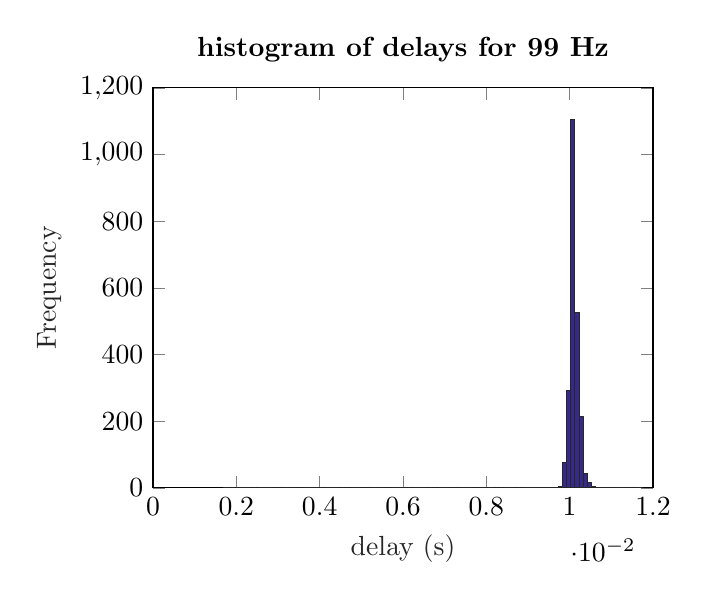
\begin{tikzpicture}

\begin{axis}[%
width=2.5in,
height=2in,
scale only axis,
point meta min=1,
point meta max=2,
colormap={mymap}{[1pt] rgb(0pt)=(0.2081,0.1663,0.5292); rgb(1pt)=(0.211624,0.189781,0.577676); rgb(2pt)=(0.212252,0.213771,0.626971); rgb(3pt)=(0.2081,0.2386,0.677086); rgb(4pt)=(0.195905,0.264457,0.7279); rgb(5pt)=(0.170729,0.291938,0.779248); rgb(6pt)=(0.125271,0.324243,0.830271); rgb(7pt)=(0.0591333,0.359833,0.868333); rgb(8pt)=(0.0116952,0.38751,0.881957); rgb(9pt)=(0.00595714,0.408614,0.882843); rgb(10pt)=(0.0165143,0.4266,0.878633); rgb(11pt)=(0.0328524,0.443043,0.871957); rgb(12pt)=(0.0498143,0.458571,0.864057); rgb(13pt)=(0.0629333,0.47369,0.855438); rgb(14pt)=(0.0722667,0.488667,0.8467); rgb(15pt)=(0.0779429,0.503986,0.838371); rgb(16pt)=(0.0793476,0.520024,0.831181); rgb(17pt)=(0.0749429,0.537543,0.826271); rgb(18pt)=(0.0640571,0.556986,0.823957); rgb(19pt)=(0.0487714,0.577224,0.822829); rgb(20pt)=(0.0343429,0.596581,0.819852); rgb(21pt)=(0.0265,0.6137,0.8135); rgb(22pt)=(0.0238905,0.628662,0.803762); rgb(23pt)=(0.0230905,0.641786,0.791267); rgb(24pt)=(0.0227714,0.653486,0.776757); rgb(25pt)=(0.0266619,0.664195,0.760719); rgb(26pt)=(0.0383714,0.674271,0.743552); rgb(27pt)=(0.0589714,0.683757,0.725386); rgb(28pt)=(0.0843,0.692833,0.706167); rgb(29pt)=(0.113295,0.7015,0.685857); rgb(30pt)=(0.145271,0.709757,0.664629); rgb(31pt)=(0.180133,0.717657,0.642433); rgb(32pt)=(0.217829,0.725043,0.619262); rgb(33pt)=(0.258643,0.731714,0.595429); rgb(34pt)=(0.302171,0.737605,0.571186); rgb(35pt)=(0.348167,0.742433,0.547267); rgb(36pt)=(0.395257,0.7459,0.524443); rgb(37pt)=(0.44201,0.748081,0.503314); rgb(38pt)=(0.487124,0.749062,0.483976); rgb(39pt)=(0.530029,0.749114,0.466114); rgb(40pt)=(0.570857,0.748519,0.44939); rgb(41pt)=(0.609852,0.747314,0.433686); rgb(42pt)=(0.6473,0.7456,0.4188); rgb(43pt)=(0.683419,0.743476,0.404433); rgb(44pt)=(0.71841,0.741133,0.390476); rgb(45pt)=(0.752486,0.7384,0.376814); rgb(46pt)=(0.785843,0.735567,0.363271); rgb(47pt)=(0.818505,0.732733,0.34979); rgb(48pt)=(0.850657,0.7299,0.336029); rgb(49pt)=(0.882433,0.727433,0.3217); rgb(50pt)=(0.913933,0.725786,0.306276); rgb(51pt)=(0.944957,0.726114,0.288643); rgb(52pt)=(0.973895,0.731395,0.266648); rgb(53pt)=(0.993771,0.745457,0.240348); rgb(54pt)=(0.999043,0.765314,0.216414); rgb(55pt)=(0.995533,0.786057,0.196652); rgb(56pt)=(0.988,0.8066,0.179367); rgb(57pt)=(0.978857,0.827143,0.163314); rgb(58pt)=(0.9697,0.848138,0.147452); rgb(59pt)=(0.962586,0.870514,0.1309); rgb(60pt)=(0.958871,0.8949,0.113243); rgb(61pt)=(0.959824,0.921833,0.0948381); rgb(62pt)=(0.9661,0.951443,0.0755333); rgb(63pt)=(0.9763,0.9831,0.0538)},
xmin=0,
xmax=0.012,
xlabel style={font=\color{white!15!black}},
xlabel={delay (s)},
ymin=0,
ymax=1200,
ylabel style={font=\color{white!15!black}},
ylabel={Frequency},
axis background/.style={fill=white},
title style={font=\bfseries},
title={histogram of delays for 99 Hz}
]

\addplot[area legend, table/row sep=crcr, patch, patch type=rectangle, shader=flat corner, draw=white!15!black, forget plot, patch table with point meta={%
1	2	3	4	1\\
6	7	8	9	1\\
11	12	13	14	1\\
16	17	18	19	1\\
21	22	23	24	1\\
26	27	28	29	1\\
31	32	33	34	1\\
36	37	38	39	1\\
41	42	43	44	1\\
46	47	48	49	1\\
51	52	53	54	1\\
56	57	58	59	1\\
61	62	63	64	1\\
66	67	68	69	1\\
71	72	73	74	1\\
76	77	78	79	1\\
81	82	83	84	1\\
86	87	88	89	1\\
91	92	93	94	1\\
96	97	98	99	1\\
101	102	103	104	1\\
106	107	108	109	1\\
111	112	113	114	1\\
116	117	118	119	1\\
121	122	123	124	1\\
126	127	128	129	1\\
131	132	133	134	1\\
136	137	138	139	1\\
141	142	143	144	1\\
146	147	148	149	1\\
151	152	153	154	1\\
156	157	158	159	1\\
161	162	163	164	1\\
166	167	168	169	1\\
171	172	173	174	1\\
176	177	178	179	1\\
181	182	183	184	1\\
186	187	188	189	1\\
191	192	193	194	1\\
196	197	198	199	1\\
201	202	203	204	1\\
206	207	208	209	1\\
211	212	213	214	1\\
216	217	218	219	1\\
221	222	223	224	1\\
226	227	228	229	1\\
231	232	233	234	1\\
236	237	238	239	1\\
241	242	243	244	1\\
246	247	248	249	1\\
251	252	253	254	1\\
256	257	258	259	1\\
261	262	263	264	1\\
266	267	268	269	1\\
271	272	273	274	1\\
276	277	278	279	1\\
281	282	283	284	1\\
286	287	288	289	1\\
291	292	293	294	1\\
296	297	298	299	1\\
301	302	303	304	1\\
306	307	308	309	1\\
311	312	313	314	1\\
316	317	318	319	1\\
321	322	323	324	1\\
326	327	328	329	1\\
331	332	333	334	1\\
336	337	338	339	1\\
341	342	343	344	1\\
346	347	348	349	1\\
351	352	353	354	1\\
356	357	358	359	1\\
361	362	363	364	1\\
366	367	368	369	1\\
371	372	373	374	1\\
376	377	378	379	1\\
381	382	383	384	1\\
386	387	388	389	1\\
391	392	393	394	1\\
396	397	398	399	1\\
401	402	403	404	1\\
406	407	408	409	1\\
411	412	413	414	1\\
416	417	418	419	1\\
421	422	423	424	1\\
426	427	428	429	1\\
431	432	433	434	1\\
436	437	438	439	1\\
441	442	443	444	1\\
446	447	448	449	1\\
451	452	453	454	1\\
456	457	458	459	1\\
461	462	463	464	1\\
466	467	468	469	1\\
471	472	473	474	1\\
476	477	478	479	1\\
481	482	483	484	1\\
486	487	488	489	1\\
491	492	493	494	1\\
496	497	498	499	1\\
}]
table[row sep=crcr] {%
x	y\\
0.001682	0\\
0.001682	0\\
0.001682	1\\
0.00178253	1\\
0.00178253	0\\
0.00178253	0\\
0.00178253	0\\
0.00178253	0\\
0.00188306	0\\
0.00188306	0\\
0.00188306	0\\
0.00188306	0\\
0.00188306	0\\
0.00198359	0\\
0.00198359	0\\
0.00198359	0\\
0.00198359	0\\
0.00198359	0\\
0.00208412	0\\
0.00208412	0\\
0.00208412	0\\
0.00208412	0\\
0.00208412	0\\
0.00218465	0\\
0.00218465	0\\
0.00218465	0\\
0.00218465	0\\
0.00218465	0\\
0.00228518	0\\
0.00228518	0\\
0.00228518	0\\
0.00228518	0\\
0.00228518	0\\
0.00238571	0\\
0.00238571	0\\
0.00238571	0\\
0.00238571	0\\
0.00238571	0\\
0.00248624	0\\
0.00248624	0\\
0.00248624	0\\
0.00248624	0\\
0.00248624	0\\
0.00258677	0\\
0.00258677	0\\
0.00258677	0\\
0.00258677	0\\
0.00258677	0\\
0.00268730000000001	0\\
0.00268730000000001	0\\
0.0026873	0\\
0.0026873	0\\
0.0026873	0\\
0.00278783000000001	0\\
0.00278783000000001	0\\
0.00278783000000001	0\\
0.00278783000000001	0\\
0.00278783000000001	0\\
0.00288836000000001	0\\
0.00288836000000001	0\\
0.00288836000000001	0\\
0.00288836000000001	0\\
0.00288836000000001	0\\
0.00298889000000001	0\\
0.00298889000000001	0\\
0.00298889000000001	0\\
0.00298889000000001	0\\
0.00298889000000001	0\\
0.00308942000000001	0\\
0.00308942000000001	0\\
0.00308942000000001	0\\
0.00308942000000001	0\\
0.00308942000000001	0\\
0.00318995000000001	0\\
0.00318995000000001	0\\
0.00318995000000001	0\\
0.00318995000000001	0\\
0.00318995000000001	0\\
0.00329048000000001	0\\
0.00329048000000001	0\\
0.00329048000000001	0\\
0.00329048000000001	0\\
0.00329048000000001	0\\
0.00339101000000001	0\\
0.00339101000000001	0\\
0.00339101000000001	0\\
0.00339101000000001	0\\
0.00339101000000001	0\\
0.00349154000000001	0\\
0.00349154000000001	0\\
0.00349154000000001	0\\
0.00349154000000001	0\\
0.00349154000000001	0\\
0.00359207000000001	0\\
0.00359207000000001	0\\
0.00359207000000001	0\\
0.00359207000000001	0\\
0.00359207000000001	0\\
0.00369260000000001	0\\
0.00369260000000001	0\\
0.00369260000000001	0\\
0.00369260000000001	0\\
0.00369260000000001	0\\
0.00379313000000001	0\\
0.00379313000000001	0\\
0.00379313000000001	0\\
0.00379313000000001	0\\
0.00379313000000001	0\\
0.00389366000000001	0\\
0.00389366000000001	0\\
0.00389366000000001	0\\
0.00389366000000001	0\\
0.00389366000000001	0\\
0.00399419000000001	0\\
0.00399419000000001	0\\
0.00399419000000001	0\\
0.00399419000000001	0\\
0.00399419000000001	0\\
0.00409472000000001	0\\
0.00409472000000001	0\\
0.00409472000000001	0\\
0.00409472000000001	0\\
0.00409472000000001	0\\
0.00419525000000001	0\\
0.00419525000000001	0\\
0.00419525000000001	0\\
0.00419525000000001	0\\
0.00419525000000001	0\\
0.00429578000000001	0\\
0.00429578000000001	0\\
0.00429578000000001	0\\
0.00429578000000001	0\\
0.00429578000000001	0\\
0.00439631000000001	0\\
0.00439631000000001	0\\
0.00439631000000001	0\\
0.00439631000000001	0\\
0.00439631000000001	0\\
0.00449684000000001	0\\
0.00449684000000001	0\\
0.00449684000000001	0\\
0.00449684000000001	0\\
0.00449684000000001	0\\
0.00459737000000002	0\\
0.00459737000000002	0\\
0.00459737000000001	0\\
0.00459737000000001	0\\
0.00459737000000001	0\\
0.00469790000000002	0\\
0.00469790000000002	0\\
0.00469790000000002	0\\
0.00469790000000002	0\\
0.00469790000000002	0\\
0.00479843000000002	0\\
0.00479843000000002	0\\
0.00479843000000002	0\\
0.00479843000000002	0\\
0.00479843000000002	0\\
0.00489896000000002	0\\
0.00489896000000002	0\\
0.00489896000000002	0\\
0.00489896000000002	0\\
0.00489896000000002	0\\
0.00499949000000002	0\\
0.00499949000000002	0\\
0.00499949000000002	0\\
0.00499949000000002	0\\
0.00499949000000002	0\\
0.00510002000000002	0\\
0.00510002000000002	0\\
0.00510002000000002	0\\
0.00510002000000002	0\\
0.00510002000000002	0\\
0.00520055000000002	0\\
0.00520055000000002	0\\
0.00520055000000002	0\\
0.00520055000000002	0\\
0.00520055000000002	0\\
0.00530108000000002	0\\
0.00530108000000002	0\\
0.00530108000000002	0\\
0.00530108000000002	0\\
0.00530108000000002	0\\
0.00540161000000002	0\\
0.00540161000000002	0\\
0.00540161000000002	0\\
0.00540161000000002	0\\
0.00540161000000002	0\\
0.00550214000000002	0\\
0.00550214000000002	0\\
0.00550214000000002	0\\
0.00550214000000002	0\\
0.00550214000000002	0\\
0.00560267000000002	0\\
0.00560267000000002	0\\
0.00560267000000002	0\\
0.00560267000000002	0\\
0.00560267000000002	0\\
0.00570320000000002	0\\
0.00570320000000002	0\\
0.00570320000000002	0\\
0.00570320000000002	0\\
0.00570320000000002	0\\
0.00580373000000002	0\\
0.00580373000000002	0\\
0.00580373000000002	0\\
0.00580373000000002	0\\
0.00580373000000002	0\\
0.00590426000000002	0\\
0.00590426000000002	0\\
0.00590426000000002	0\\
0.00590426000000002	0\\
0.00590426000000002	0\\
0.00600479000000002	0\\
0.00600479000000002	0\\
0.00600479000000002	0\\
0.00600479000000002	0\\
0.00600479000000002	0\\
0.00610532000000002	0\\
0.00610532000000002	0\\
0.00610532000000002	0\\
0.00610532000000002	0\\
0.00610532000000002	0\\
0.00620585000000002	0\\
0.00620585000000002	0\\
0.00620585000000002	0\\
0.00620585000000002	0\\
0.00620585000000002	0\\
0.00630638000000002	0\\
0.00630638000000002	0\\
0.00630638000000002	0\\
0.00630638000000002	0\\
0.00630638000000002	0\\
0.00640691000000002	0\\
0.00640691000000002	0\\
0.00640691000000003	0\\
0.00640691000000003	0\\
0.00640691000000003	0\\
0.00650744000000003	0\\
0.00650744000000003	0\\
0.00650744000000002	0\\
0.00650744000000002	0\\
0.00650744000000002	0\\
0.00660797000000003	0\\
0.00660797000000003	0\\
0.00660797000000003	0\\
0.00660797000000003	0\\
0.00660797000000003	0\\
0.00670850000000003	0\\
0.00670850000000003	0\\
0.00670850000000003	0\\
0.00670850000000003	0\\
0.00670850000000003	0\\
0.00680903000000003	0\\
0.00680903000000003	0\\
0.00680903000000003	0\\
0.00680903000000003	0\\
0.00680903000000003	0\\
0.00690956000000003	0\\
0.00690956000000003	0\\
0.00690956000000003	0\\
0.00690956000000003	0\\
0.00690956000000003	0\\
0.00701009000000003	0\\
0.00701009000000003	0\\
0.00701009000000003	0\\
0.00701009000000003	0\\
0.00701009000000003	0\\
0.00711062000000003	0\\
0.00711062000000003	0\\
0.00711062000000003	0\\
0.00711062000000003	0\\
0.00711062000000003	0\\
0.00721115000000003	0\\
0.00721115000000003	0\\
0.00721115000000003	0\\
0.00721115000000003	0\\
0.00721115000000003	0\\
0.00731168000000003	0\\
0.00731168000000003	0\\
0.00731168000000003	0\\
0.00731168000000003	0\\
0.00731168000000003	0\\
0.00741221000000003	0\\
0.00741221000000003	0\\
0.00741221000000003	0\\
0.00741221000000003	0\\
0.00741221000000003	0\\
0.00751274000000003	0\\
0.00751274000000003	0\\
0.00751274000000003	0\\
0.00751274000000003	0\\
0.00751274000000003	0\\
0.00761327000000003	0\\
0.00761327000000003	0\\
0.00761327000000003	0\\
0.00761327000000003	0\\
0.00761327000000003	0\\
0.00771380000000003	0\\
0.00771380000000003	0\\
0.00771380000000003	0\\
0.00771380000000003	0\\
0.00771380000000003	0\\
0.00781433000000003	0\\
0.00781433000000003	0\\
0.00781433000000003	0\\
0.00781433000000003	0\\
0.00781433000000003	0\\
0.00791486000000003	0\\
0.00791486000000003	0\\
0.00791486000000003	0\\
0.00791486000000003	0\\
0.00791486000000003	0\\
0.00801539000000003	0\\
0.00801539000000003	0\\
0.00801539000000003	0\\
0.00801539000000003	0\\
0.00801539000000003	0\\
0.00811592000000003	0\\
0.00811592000000003	0\\
0.00811592000000003	0\\
0.00811592000000003	0\\
0.00811592000000003	0\\
0.00821645000000003	0\\
0.00821645000000003	0\\
0.00821645000000003	0\\
0.00821645000000003	0\\
0.00821645000000003	0\\
0.00831698000000003	0\\
0.00831698000000003	0\\
0.00831698000000003	0\\
0.00831698000000003	0\\
0.00831698000000003	0\\
0.00841751000000003	0\\
0.00841751000000003	0\\
0.00841751000000003	0\\
0.00841751000000003	0\\
0.00841751000000003	0\\
0.00851804000000003	0\\
0.00851804000000003	0\\
0.00851804000000004	0\\
0.00851804000000004	0\\
0.00851804000000004	0\\
0.00861857000000004	0\\
0.00861857000000004	0\\
0.00861857000000004	0\\
0.00861857000000004	0\\
0.00861857000000004	0\\
0.00871910000000004	0\\
0.00871910000000004	0\\
0.00871910000000004	0\\
0.00871910000000004	0\\
0.00871910000000004	0\\
0.00881963000000003	0\\
0.00881963000000003	0\\
0.00881963000000004	0\\
0.00881963000000004	0\\
0.00881963000000004	0\\
0.00892016000000004	0\\
0.00892016000000004	0\\
0.00892016000000004	0\\
0.00892016000000004	0\\
0.00892016000000004	1\\
0.00902069000000004	1\\
0.00902069000000004	0\\
0.00902069000000004	0\\
0.00902069000000004	0\\
0.00902069000000004	1\\
0.00912122000000004	1\\
0.00912122000000004	0\\
0.00912122000000004	0\\
0.00912122000000004	0\\
0.00912122000000004	0\\
0.00922175000000004	0\\
0.00922175000000004	0\\
0.00922175000000004	0\\
0.00922175000000004	0\\
0.00922175000000004	1\\
0.00932228000000004	1\\
0.00932228000000004	0\\
0.00932228000000004	0\\
0.00932228000000004	0\\
0.00932228000000004	1\\
0.00942281000000004	1\\
0.00942281000000004	0\\
0.00942281000000004	0\\
0.00942281000000004	0\\
0.00942281000000004	0\\
0.00952334000000004	0\\
0.00952334000000004	0\\
0.00952334000000004	0\\
0.00952334000000004	0\\
0.00952334000000004	0\\
0.00962387000000004	0\\
0.00962387000000004	0\\
0.00962387000000004	0\\
0.00962387000000004	0\\
0.00962387000000004	0\\
0.00972440000000004	0\\
0.00972440000000004	0\\
0.00972440000000004	0\\
0.00972440000000004	0\\
0.00972440000000004	4\\
0.00982493000000004	4\\
0.00982493000000004	0\\
0.00982493000000004	0\\
0.00982493000000004	0\\
0.00982493000000004	75\\
0.00992546000000004	75\\
0.00992546000000004	0\\
0.00992546000000004	0\\
0.00992546000000004	0\\
0.00992546000000004	293\\
0.01002599	293\\
0.01002599	0\\
0.01002599	0\\
0.01002599	0\\
0.01002599	1106\\
0.01012652	1106\\
0.01012652	0\\
0.01012652	0\\
0.01012652	0\\
0.01012652	525\\
0.01022705	525\\
0.01022705	0\\
0.01022705	0\\
0.01022705	0\\
0.01022705	214\\
0.01032758	214\\
0.01032758	0\\
0.01032758	0\\
0.01032758	0\\
0.01032758	44\\
0.01042811	44\\
0.01042811	0\\
0.01042811	0\\
0.01042811	0\\
0.01042811	15\\
0.01052864	15\\
0.01052864	0\\
0.01052864	0\\
0.01052864	0\\
0.01052864	3\\
0.01062917	3\\
0.01062917	0\\
0.01062917	0\\
0.01062917	0\\
0.01062917	1\\
0.0107297	1\\
0.0107297	0\\
0.0107297	0\\
0.0107297	0\\
0.0107297	1\\
0.01083023	1\\
0.01083023	0\\
0.01083023	0\\
0.01083023	0\\
0.01083023	0\\
0.01093076	0\\
0.01093076	0\\
0.01093076	0\\
0.01093076	0\\
0.01093076	1\\
0.01103129	1\\
0.01103129	0\\
0.01103129	0\\
0.01103129	0\\
0.01103129	0\\
0.01113182	0\\
0.01113182	0\\
0.01113182	0\\
0.01113182	0\\
0.01113182	1\\
0.01123235	1\\
0.01123235	0\\
0.01123235	0\\
0.01123235	0\\
0.01123235	2\\
0.01133288	2\\
0.01133288	0\\
0.01133288	0\\
0.01133288	0\\
0.01133288	0\\
0.01143341	0\\
0.01143341	0\\
0.0114334100000001	0\\
0.0114334100000001	0\\
0.0114334100000001	0\\
0.01153394	0\\
0.01153394	0\\
0.01153394	0\\
0.01153394	0\\
0.01153394	0\\
0.01163447	0\\
0.01163447	0\\
0.0116344700000001	0\\
0.0116344700000001	0\\
0.0116344700000001	1\\
0.0117350000000001	1\\
0.0117350000000001	0\\
0.0117350000000001	0\\
};
\end{axis}
\end{tikzpicture}%
% 	    \caption{10ms}
% 	\end{subfigure} 
% 	\begin{subfigure}{.45\textwidth}
% 	    \centering
% 	    % This file was created by matlab2tikz.
%
%The latest updates can be retrieved from
%  http://www.mathworks.com/matlabcentral/fileexchange/22022-matlab2tikz-matlab2tikz
%where you can also make suggestions and rate matlab2tikz.
%
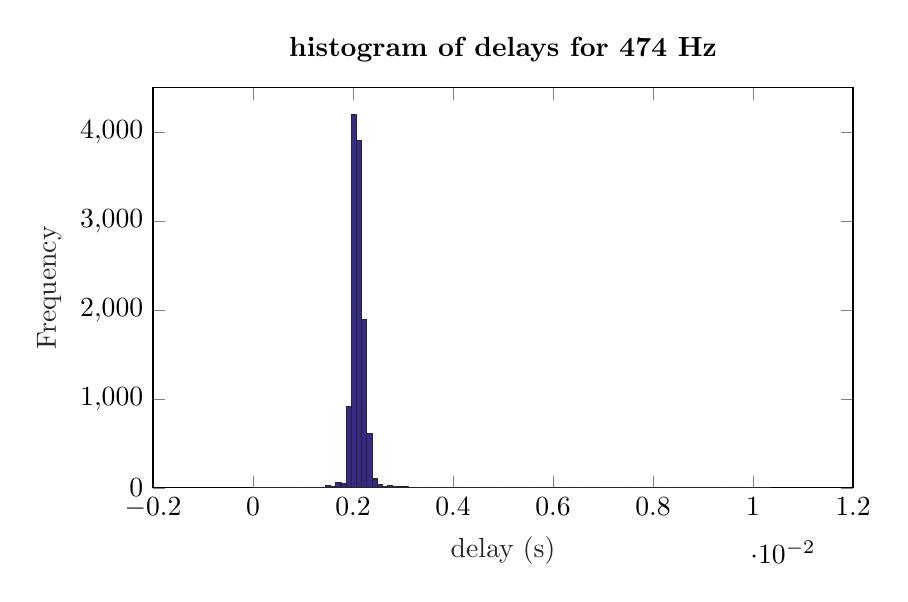
\begin{tikzpicture}

\begin{axis}[%
width=3.5in,
height=2in,
scale only axis,
point meta min=1,
point meta max=2,
colormap={mymap}{[1pt] rgb(0pt)=(0.2081,0.1663,0.5292); rgb(1pt)=(0.211624,0.189781,0.577676); rgb(2pt)=(0.212252,0.213771,0.626971); rgb(3pt)=(0.2081,0.2386,0.677086); rgb(4pt)=(0.195905,0.264457,0.7279); rgb(5pt)=(0.170729,0.291938,0.779248); rgb(6pt)=(0.125271,0.324243,0.830271); rgb(7pt)=(0.0591333,0.359833,0.868333); rgb(8pt)=(0.0116952,0.38751,0.881957); rgb(9pt)=(0.00595714,0.408614,0.882843); rgb(10pt)=(0.0165143,0.4266,0.878633); rgb(11pt)=(0.0328524,0.443043,0.871957); rgb(12pt)=(0.0498143,0.458571,0.864057); rgb(13pt)=(0.0629333,0.47369,0.855438); rgb(14pt)=(0.0722667,0.488667,0.8467); rgb(15pt)=(0.0779429,0.503986,0.838371); rgb(16pt)=(0.0793476,0.520024,0.831181); rgb(17pt)=(0.0749429,0.537543,0.826271); rgb(18pt)=(0.0640571,0.556986,0.823957); rgb(19pt)=(0.0487714,0.577224,0.822829); rgb(20pt)=(0.0343429,0.596581,0.819852); rgb(21pt)=(0.0265,0.6137,0.8135); rgb(22pt)=(0.0238905,0.628662,0.803762); rgb(23pt)=(0.0230905,0.641786,0.791267); rgb(24pt)=(0.0227714,0.653486,0.776757); rgb(25pt)=(0.0266619,0.664195,0.760719); rgb(26pt)=(0.0383714,0.674271,0.743552); rgb(27pt)=(0.0589714,0.683757,0.725386); rgb(28pt)=(0.0843,0.692833,0.706167); rgb(29pt)=(0.113295,0.7015,0.685857); rgb(30pt)=(0.145271,0.709757,0.664629); rgb(31pt)=(0.180133,0.717657,0.642433); rgb(32pt)=(0.217829,0.725043,0.619262); rgb(33pt)=(0.258643,0.731714,0.595429); rgb(34pt)=(0.302171,0.737605,0.571186); rgb(35pt)=(0.348167,0.742433,0.547267); rgb(36pt)=(0.395257,0.7459,0.524443); rgb(37pt)=(0.44201,0.748081,0.503314); rgb(38pt)=(0.487124,0.749062,0.483976); rgb(39pt)=(0.530029,0.749114,0.466114); rgb(40pt)=(0.570857,0.748519,0.44939); rgb(41pt)=(0.609852,0.747314,0.433686); rgb(42pt)=(0.6473,0.7456,0.4188); rgb(43pt)=(0.683419,0.743476,0.404433); rgb(44pt)=(0.71841,0.741133,0.390476); rgb(45pt)=(0.752486,0.7384,0.376814); rgb(46pt)=(0.785843,0.735567,0.363271); rgb(47pt)=(0.818505,0.732733,0.34979); rgb(48pt)=(0.850657,0.7299,0.336029); rgb(49pt)=(0.882433,0.727433,0.3217); rgb(50pt)=(0.913933,0.725786,0.306276); rgb(51pt)=(0.944957,0.726114,0.288643); rgb(52pt)=(0.973895,0.731395,0.266648); rgb(53pt)=(0.993771,0.745457,0.240348); rgb(54pt)=(0.999043,0.765314,0.216414); rgb(55pt)=(0.995533,0.786057,0.196652); rgb(56pt)=(0.988,0.8066,0.179367); rgb(57pt)=(0.978857,0.827143,0.163314); rgb(58pt)=(0.9697,0.848138,0.147452); rgb(59pt)=(0.962586,0.870514,0.1309); rgb(60pt)=(0.958871,0.8949,0.113243); rgb(61pt)=(0.959824,0.921833,0.0948381); rgb(62pt)=(0.9661,0.951443,0.0755333); rgb(63pt)=(0.9763,0.9831,0.0538)},
xmin=-0.002,
xmax=0.012,
xlabel style={font=\color{white!15!black}},
xlabel={delay (s)},
ymin=0,
ymax=4500,
ylabel style={font=\color{white!15!black}},
ylabel={Frequency},
axis background/.style={fill=white},
title style={font=\bfseries},
title={histogram of delays for 474 Hz}
]

\addplot[area legend, table/row sep=crcr, patch, patch type=rectangle, shader=flat corner, draw=white!15!black, forget plot, patch table with point meta={%
1	2	3	4	1\\
6	7	8	9	1\\
11	12	13	14	1\\
16	17	18	19	1\\
21	22	23	24	1\\
26	27	28	29	1\\
31	32	33	34	1\\
36	37	38	39	1\\
41	42	43	44	1\\
46	47	48	49	1\\
51	52	53	54	1\\
56	57	58	59	1\\
61	62	63	64	1\\
66	67	68	69	1\\
71	72	73	74	1\\
76	77	78	79	1\\
81	82	83	84	1\\
86	87	88	89	1\\
91	92	93	94	1\\
96	97	98	99	1\\
101	102	103	104	1\\
106	107	108	109	1\\
111	112	113	114	1\\
116	117	118	119	1\\
121	122	123	124	1\\
126	127	128	129	1\\
131	132	133	134	1\\
136	137	138	139	1\\
141	142	143	144	1\\
146	147	148	149	1\\
151	152	153	154	1\\
156	157	158	159	1\\
161	162	163	164	1\\
166	167	168	169	1\\
171	172	173	174	1\\
176	177	178	179	1\\
181	182	183	184	1\\
186	187	188	189	1\\
191	192	193	194	1\\
196	197	198	199	1\\
201	202	203	204	1\\
206	207	208	209	1\\
211	212	213	214	1\\
216	217	218	219	1\\
221	222	223	224	1\\
226	227	228	229	1\\
231	232	233	234	1\\
236	237	238	239	1\\
241	242	243	244	1\\
246	247	248	249	1\\
251	252	253	254	1\\
256	257	258	259	1\\
261	262	263	264	1\\
266	267	268	269	1\\
271	272	273	274	1\\
276	277	278	279	1\\
281	282	283	284	1\\
286	287	288	289	1\\
291	292	293	294	1\\
296	297	298	299	1\\
301	302	303	304	1\\
306	307	308	309	1\\
311	312	313	314	1\\
316	317	318	319	1\\
321	322	323	324	1\\
326	327	328	329	1\\
331	332	333	334	1\\
336	337	338	339	1\\
341	342	343	344	1\\
346	347	348	349	1\\
351	352	353	354	1\\
356	357	358	359	1\\
361	362	363	364	1\\
366	367	368	369	1\\
371	372	373	374	1\\
376	377	378	379	1\\
381	382	383	384	1\\
386	387	388	389	1\\
391	392	393	394	1\\
396	397	398	399	1\\
401	402	403	404	1\\
406	407	408	409	1\\
411	412	413	414	1\\
416	417	418	419	1\\
421	422	423	424	1\\
426	427	428	429	1\\
431	432	433	434	1\\
436	437	438	439	1\\
441	442	443	444	1\\
446	447	448	449	1\\
451	452	453	454	1\\
456	457	458	459	1\\
461	462	463	464	1\\
466	467	468	469	1\\
471	472	473	474	1\\
476	477	478	479	1\\
481	482	483	484	1\\
486	487	488	489	1\\
491	492	493	494	1\\
496	497	498	499	1\\
}]
table[row sep=crcr] {%
x	y\\
-6.7762635780344e-21	0\\
-6.7762635780344e-21	0\\
-6.7762635780344e-21	1\\
0.000103580000000001	1\\
0.000103580000000001	0\\
0.000103580000000001	0\\
0.000103580000000001	0\\
0.000103580000000001	0\\
0.000207160000000002	0\\
0.000207160000000002	0\\
0.000207160000000002	0\\
0.000207160000000002	0\\
0.000207160000000002	0\\
0.000310740000000003	0\\
0.000310740000000003	0\\
0.000310740000000003	0\\
0.000310740000000003	0\\
0.000310740000000003	0\\
0.000414320000000004	0\\
0.000414320000000004	0\\
0.000414320000000004	0\\
0.000414320000000004	0\\
0.000414320000000004	0\\
0.000517900000000005	0\\
0.000517900000000005	0\\
0.000517900000000005	0\\
0.000517900000000005	0\\
0.000517900000000005	0\\
0.000621480000000005	0\\
0.000621480000000005	0\\
0.000621480000000005	0\\
0.000621480000000005	0\\
0.000621480000000005	0\\
0.000725060000000006	0\\
0.000725060000000006	0\\
0.000725060000000006	0\\
0.000725060000000006	0\\
0.000725060000000006	0\\
0.000828640000000007	0\\
0.000828640000000007	0\\
0.000828640000000007	0\\
0.000828640000000007	0\\
0.000828640000000007	0\\
0.000932220000000008	0\\
0.000932220000000008	0\\
0.000932220000000008	0\\
0.000932220000000008	0\\
0.000932220000000008	0\\
0.00103580000000001	0\\
0.00103580000000001	0\\
0.00103580000000001	0\\
0.00103580000000001	0\\
0.00103580000000001	0\\
0.00113938000000001	0\\
0.00113938000000001	0\\
0.00113938000000001	0\\
0.00113938000000001	0\\
0.00113938000000001	0\\
0.00124296000000001	0\\
0.00124296000000001	0\\
0.00124296000000001	0\\
0.00124296000000001	0\\
0.00124296000000001	0\\
0.00134654000000001	0\\
0.00134654000000001	0\\
0.00134654000000001	0\\
0.00134654000000001	0\\
0.00134654000000001	9\\
0.00145012000000001	9\\
0.00145012000000001	0\\
0.00145012000000001	0\\
0.00145012000000001	0\\
0.00145012000000001	28\\
0.00155370000000001	28\\
0.00155370000000001	0\\
0.00155370000000001	0\\
0.00155370000000001	0\\
0.00155370000000001	18\\
0.00165728000000001	18\\
0.00165728000000001	0\\
0.00165728000000001	0\\
0.00165728000000001	0\\
0.00165728000000001	56\\
0.00176086000000001	56\\
0.00176086000000001	0\\
0.00176086000000002	0\\
0.00176086000000002	0\\
0.00176086000000002	45\\
0.00186444000000002	45\\
0.00186444000000002	0\\
0.00186444000000002	0\\
0.00186444000000002	0\\
0.00186444000000002	916\\
0.00196802000000002	916\\
0.00196802000000002	0\\
0.00196802000000002	0\\
0.00196802000000002	0\\
0.00196802000000002	4199\\
0.00207160000000002	4199\\
0.00207160000000002	0\\
0.00207160000000002	0\\
0.00207160000000002	0\\
0.00207160000000002	3910\\
0.00217518000000002	3910\\
0.00217518000000002	0\\
0.00217518000000002	0\\
0.00217518000000002	0\\
0.00217518000000002	1896\\
0.00227876000000002	1896\\
0.00227876000000002	0\\
0.00227876000000002	0\\
0.00227876000000002	0\\
0.00227876000000002	608\\
0.00238234000000002	608\\
0.00238234000000002	0\\
0.00238234000000002	0\\
0.00238234000000002	0\\
0.00238234000000002	100\\
0.00248592000000002	100\\
0.00248592000000002	0\\
0.00248592000000002	0\\
0.00248592000000002	0\\
0.00248592000000002	37\\
0.00258950000000002	37\\
0.00258950000000002	0\\
0.00258950000000002	0\\
0.00258950000000002	0\\
0.00258950000000002	15\\
0.00269308000000002	15\\
0.00269308000000002	0\\
0.00269308000000002	0\\
0.00269308000000002	0\\
0.00269308000000002	22\\
0.00279666000000002	22\\
0.00279666000000002	0\\
0.00279666000000002	0\\
0.00279666000000002	0\\
0.00279666000000002	10\\
0.00290024000000003	10\\
0.00290024000000003	0\\
0.00290024000000002	0\\
0.00290024000000002	0\\
0.00290024000000002	12\\
0.00300382000000003	12\\
0.00300382000000003	0\\
0.00300382000000003	0\\
0.00300382000000003	0\\
0.00300382000000003	10\\
0.00310740000000003	10\\
0.00310740000000003	0\\
0.00310740000000003	0\\
0.00310740000000003	0\\
0.00310740000000003	8\\
0.00321098000000003	8\\
0.00321098000000003	0\\
0.00321098000000003	0\\
0.00321098000000003	0\\
0.00321098000000003	3\\
0.00331456000000003	3\\
0.00331456000000003	0\\
0.00331456000000003	0\\
0.00331456000000003	0\\
0.00331456000000003	2\\
0.00341814000000003	2\\
0.00341814000000003	0\\
0.00341814000000003	0\\
0.00341814000000003	0\\
0.00341814000000003	2\\
0.00352172000000003	2\\
0.00352172000000003	0\\
0.00352172000000003	0\\
0.00352172000000003	0\\
0.00352172000000003	1\\
0.00362530000000003	1\\
0.00362530000000003	0\\
0.00362530000000003	0\\
0.00362530000000003	0\\
0.00362530000000003	3\\
0.00372888000000003	3\\
0.00372888000000003	0\\
0.00372888000000003	0\\
0.00372888000000003	0\\
0.00372888000000003	1\\
0.00383246000000003	1\\
0.00383246000000003	0\\
0.00383246000000003	0\\
0.00383246000000003	0\\
0.00383246000000003	3\\
0.00393604000000003	3\\
0.00393604000000003	0\\
0.00393604000000003	0\\
0.00393604000000003	0\\
0.00393604000000003	2\\
0.00403962000000003	2\\
0.00403962000000003	0\\
0.00403962000000003	0\\
0.00403962000000003	0\\
0.00403962000000003	1\\
0.00414320000000004	1\\
0.00414320000000004	0\\
0.00414320000000004	0\\
0.00414320000000004	0\\
0.00414320000000004	3\\
0.00424678000000004	3\\
0.00424678000000004	0\\
0.00424678000000004	0\\
0.00424678000000004	0\\
0.00424678000000004	1\\
0.00435036000000004	1\\
0.00435036000000004	0\\
0.00435036000000004	0\\
0.00435036000000004	0\\
0.00435036000000004	0\\
0.00445394000000004	0\\
0.00445394000000004	0\\
0.00445394000000004	0\\
0.00445394000000004	0\\
0.00445394000000004	0\\
0.00455752000000004	0\\
0.00455752000000004	0\\
0.00455752000000004	0\\
0.00455752000000004	0\\
0.00455752000000004	0\\
0.00466110000000004	0\\
0.00466110000000004	0\\
0.00466110000000004	0\\
0.00466110000000004	0\\
0.00466110000000004	0\\
0.00476468000000004	0\\
0.00476468000000004	0\\
0.00476468000000004	0\\
0.00476468000000004	0\\
0.00476468000000004	0\\
0.00486826000000004	0\\
0.00486826000000004	0\\
0.00486826000000004	0\\
0.00486826000000004	0\\
0.00486826000000004	1\\
0.00497184000000004	1\\
0.00497184000000004	0\\
0.00497184000000004	0\\
0.00497184000000004	0\\
0.00497184000000004	0\\
0.00507542000000004	0\\
0.00507542000000004	0\\
0.00507542000000004	0\\
0.00507542000000004	0\\
0.00507542000000004	1\\
0.00517900000000004	1\\
0.00517900000000004	0\\
0.00517900000000004	0\\
0.00517900000000004	0\\
0.00517900000000004	0\\
0.00528258000000005	0\\
0.00528258000000005	0\\
0.00528258000000005	0\\
0.00528258000000005	0\\
0.00528258000000005	0\\
0.00538616000000005	0\\
0.00538616000000005	0\\
0.00538616000000005	0\\
0.00538616000000005	0\\
0.00538616000000005	0\\
0.00548974000000005	0\\
0.00548974000000005	0\\
0.00548974000000005	0\\
0.00548974000000005	0\\
0.00548974000000005	0\\
0.00559332000000005	0\\
0.00559332000000005	0\\
0.00559332000000005	0\\
0.00559332000000005	0\\
0.00559332000000005	1\\
0.00569690000000005	1\\
0.00569690000000005	0\\
0.00569690000000005	0\\
0.00569690000000005	0\\
0.00569690000000005	2\\
0.00580048000000005	2\\
0.00580048000000005	0\\
0.00580048000000005	0\\
0.00580048000000005	0\\
0.00580048000000005	1\\
0.00590406000000005	1\\
0.00590406000000005	0\\
0.00590406000000005	0\\
0.00590406000000005	0\\
0.00590406000000005	1\\
0.00600764000000005	1\\
0.00600764000000005	0\\
0.00600764000000005	0\\
0.00600764000000005	0\\
0.00600764000000005	0\\
0.00611122000000005	0\\
0.00611122000000005	0\\
0.00611122000000005	0\\
0.00611122000000005	0\\
0.00611122000000005	0\\
0.00621480000000005	0\\
0.00621480000000005	0\\
0.00621480000000005	0\\
0.00621480000000005	0\\
0.00621480000000005	0\\
0.00631838000000005	0\\
0.00631838000000005	0\\
0.00631838000000005	0\\
0.00631838000000005	0\\
0.00631838000000005	0\\
0.00642196000000006	0\\
0.00642196000000006	0\\
0.00642196000000006	0\\
0.00642196000000006	0\\
0.00642196000000006	0\\
0.00652554000000006	0\\
0.00652554000000006	0\\
0.00652554000000006	0\\
0.00652554000000006	0\\
0.00652554000000006	1\\
0.00662912000000006	1\\
0.00662912000000006	0\\
0.00662912000000006	0\\
0.00662912000000006	0\\
0.00662912000000006	0\\
0.00673270000000006	0\\
0.00673270000000006	0\\
0.00673270000000006	0\\
0.00673270000000006	0\\
0.00673270000000006	0\\
0.00683628000000006	0\\
0.00683628000000006	0\\
0.00683628000000006	0\\
0.00683628000000006	0\\
0.00683628000000006	0\\
0.00693986000000006	0\\
0.00693986000000006	0\\
0.00693986000000006	0\\
0.00693986000000006	0\\
0.00693986000000006	0\\
0.00704344000000006	0\\
0.00704344000000006	0\\
0.00704344000000006	0\\
0.00704344000000006	0\\
0.00704344000000006	1\\
0.00714702000000006	1\\
0.00714702000000006	0\\
0.00714702000000006	0\\
0.00714702000000006	0\\
0.00714702000000006	0\\
0.00725060000000006	0\\
0.00725060000000006	0\\
0.00725060000000006	0\\
0.00725060000000006	0\\
0.00725060000000006	1\\
0.00735418000000006	1\\
0.00735418000000006	0\\
0.00735418000000006	0\\
0.00735418000000006	0\\
0.00735418000000006	0\\
0.00745776000000006	0\\
0.00745776000000006	0\\
0.00745776000000006	0\\
0.00745776000000006	0\\
0.00745776000000006	0\\
0.00756134000000006	0\\
0.00756134000000006	0\\
0.00756134000000007	0\\
0.00756134000000007	0\\
0.00756134000000007	0\\
0.00766492000000007	0\\
0.00766492000000007	0\\
0.00766492000000007	0\\
0.00766492000000007	0\\
0.00766492000000007	0\\
0.00776850000000007	0\\
0.00776850000000007	0\\
0.00776850000000007	0\\
0.00776850000000007	0\\
0.00776850000000007	0\\
0.00787208000000007	0\\
0.00787208000000007	0\\
0.00787208000000007	0\\
0.00787208000000007	0\\
0.00787208000000007	1\\
0.00797566000000007	1\\
0.00797566000000007	0\\
0.00797566000000007	0\\
0.00797566000000007	0\\
0.00797566000000007	0\\
0.00807924000000007	0\\
0.00807924000000007	0\\
0.00807924000000007	0\\
0.00807924000000007	0\\
0.00807924000000007	0\\
0.00818282000000007	0\\
0.00818282000000007	0\\
0.00818282000000007	0\\
0.00818282000000007	0\\
0.00818282000000007	0\\
0.00828640000000007	0\\
0.00828640000000007	0\\
0.00828640000000007	0\\
0.00828640000000007	0\\
0.00828640000000007	0\\
0.00838998000000007	0\\
0.00838998000000007	0\\
0.00838998000000007	0\\
0.00838998000000007	0\\
0.00838998000000007	0\\
0.00849356000000007	0\\
0.00849356000000007	0\\
0.00849356000000007	0\\
0.00849356000000007	0\\
0.00849356000000007	0\\
0.00859714000000007	0\\
0.00859714000000007	0\\
0.00859714000000007	0\\
0.00859714000000007	0\\
0.00859714000000007	0\\
0.00870072000000007	0\\
0.00870072000000007	0\\
0.00870072000000007	0\\
0.00870072000000007	0\\
0.00870072000000007	0\\
0.00880430000000008	0\\
0.00880430000000008	0\\
0.00880430000000008	0\\
0.00880430000000008	0\\
0.00880430000000008	0\\
0.00890788000000008	0\\
0.00890788000000008	0\\
0.00890788000000008	0\\
0.00890788000000008	0\\
0.00890788000000008	0\\
0.00901146000000008	0\\
0.00901146000000008	0\\
0.00901146000000008	0\\
0.00901146000000008	0\\
0.00901146000000008	0\\
0.00911504000000008	0\\
0.00911504000000008	0\\
0.00911504000000008	0\\
0.00911504000000008	0\\
0.00911504000000008	0\\
0.00921862000000008	0\\
0.00921862000000008	0\\
0.00921862000000008	0\\
0.00921862000000008	0\\
0.00921862000000008	0\\
0.00932220000000008	0\\
0.00932220000000008	0\\
0.00932220000000008	0\\
0.00932220000000008	0\\
0.00932220000000008	0\\
0.00942578000000008	0\\
0.00942578000000008	0\\
0.00942578000000008	0\\
0.00942578000000008	0\\
0.00942578000000008	0\\
0.00952936000000008	0\\
0.00952936000000008	0\\
0.00952936000000008	0\\
0.00952936000000008	0\\
0.00952936000000008	0\\
0.00963294000000008	0\\
0.00963294000000008	0\\
0.00963294000000008	0\\
0.00963294000000008	0\\
0.00963294000000008	0\\
0.00973652000000008	0\\
0.00973652000000008	0\\
0.00973652000000008	0\\
0.00973652000000008	0\\
0.00973652000000008	0\\
0.00984010000000008	0\\
0.00984010000000008	0\\
0.00984010000000008	0\\
0.00984010000000008	0\\
0.00984010000000008	0\\
0.00994368000000008	0\\
0.00994368000000008	0\\
0.00994368000000009	0\\
0.00994368000000009	0\\
0.00994368000000009	1\\
0.0100472600000001	1\\
0.0100472600000001	0\\
0.0100472600000001	0\\
0.0100472600000001	0\\
0.0100472600000001	1\\
0.0101508400000001	1\\
0.0101508400000001	0\\
0.0101508400000001	0\\
0.0101508400000001	0\\
0.0101508400000001	0\\
0.0102544200000001	0\\
0.0102544200000001	0\\
0.0102544200000001	0\\
0.0102544200000001	0\\
0.0102544200000001	1\\
0.0103580000000001	1\\
0.0103580000000001	0\\
0.0103580000000001	0\\
};
\end{axis}
\end{tikzpicture}%
% 	    \caption{2ms}
% 	\end{subfigure} 
% 	\begin{subfigure}{.45\textwidth}
% 	    \centering
% 	    % This file was created by matlab2tikz.
%
%The latest updates can be retrieved from
%  http://www.mathworks.com/matlabcentral/fileexchange/22022-matlab2tikz-matlab2tikz
%where you can also make suggestions and rate matlab2tikz.
%
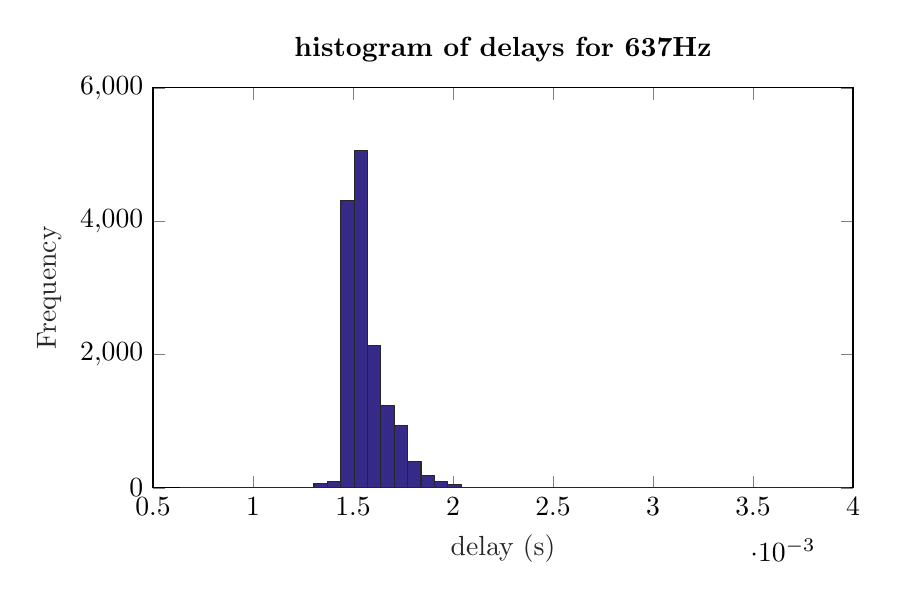
\begin{tikzpicture}

\begin{axis}[%
width=3.5in,
height=2in,
at={(1.255in,1.115in)},
scale only axis,
point meta min=1,
point meta max=2,
colormap={mymap}{[1pt] rgb(0pt)=(0.2081,0.1663,0.5292); rgb(1pt)=(0.211624,0.189781,0.577676); rgb(2pt)=(0.212252,0.213771,0.626971); rgb(3pt)=(0.2081,0.2386,0.677086); rgb(4pt)=(0.195905,0.264457,0.7279); rgb(5pt)=(0.170729,0.291938,0.779248); rgb(6pt)=(0.125271,0.324243,0.830271); rgb(7pt)=(0.0591333,0.359833,0.868333); rgb(8pt)=(0.0116952,0.38751,0.881957); rgb(9pt)=(0.00595714,0.408614,0.882843); rgb(10pt)=(0.0165143,0.4266,0.878633); rgb(11pt)=(0.0328524,0.443043,0.871957); rgb(12pt)=(0.0498143,0.458571,0.864057); rgb(13pt)=(0.0629333,0.47369,0.855438); rgb(14pt)=(0.0722667,0.488667,0.8467); rgb(15pt)=(0.0779429,0.503986,0.838371); rgb(16pt)=(0.0793476,0.520024,0.831181); rgb(17pt)=(0.0749429,0.537543,0.826271); rgb(18pt)=(0.0640571,0.556986,0.823957); rgb(19pt)=(0.0487714,0.577224,0.822829); rgb(20pt)=(0.0343429,0.596581,0.819852); rgb(21pt)=(0.0265,0.6137,0.8135); rgb(22pt)=(0.0238905,0.628662,0.803762); rgb(23pt)=(0.0230905,0.641786,0.791267); rgb(24pt)=(0.0227714,0.653486,0.776757); rgb(25pt)=(0.0266619,0.664195,0.760719); rgb(26pt)=(0.0383714,0.674271,0.743552); rgb(27pt)=(0.0589714,0.683757,0.725386); rgb(28pt)=(0.0843,0.692833,0.706167); rgb(29pt)=(0.113295,0.7015,0.685857); rgb(30pt)=(0.145271,0.709757,0.664629); rgb(31pt)=(0.180133,0.717657,0.642433); rgb(32pt)=(0.217829,0.725043,0.619262); rgb(33pt)=(0.258643,0.731714,0.595429); rgb(34pt)=(0.302171,0.737605,0.571186); rgb(35pt)=(0.348167,0.742433,0.547267); rgb(36pt)=(0.395257,0.7459,0.524443); rgb(37pt)=(0.44201,0.748081,0.503314); rgb(38pt)=(0.487124,0.749062,0.483976); rgb(39pt)=(0.530029,0.749114,0.466114); rgb(40pt)=(0.570857,0.748519,0.44939); rgb(41pt)=(0.609852,0.747314,0.433686); rgb(42pt)=(0.6473,0.7456,0.4188); rgb(43pt)=(0.683419,0.743476,0.404433); rgb(44pt)=(0.71841,0.741133,0.390476); rgb(45pt)=(0.752486,0.7384,0.376814); rgb(46pt)=(0.785843,0.735567,0.363271); rgb(47pt)=(0.818505,0.732733,0.34979); rgb(48pt)=(0.850657,0.7299,0.336029); rgb(49pt)=(0.882433,0.727433,0.3217); rgb(50pt)=(0.913933,0.725786,0.306276); rgb(51pt)=(0.944957,0.726114,0.288643); rgb(52pt)=(0.973895,0.731395,0.266648); rgb(53pt)=(0.993771,0.745457,0.240348); rgb(54pt)=(0.999043,0.765314,0.216414); rgb(55pt)=(0.995533,0.786057,0.196652); rgb(56pt)=(0.988,0.8066,0.179367); rgb(57pt)=(0.978857,0.827143,0.163314); rgb(58pt)=(0.9697,0.848138,0.147452); rgb(59pt)=(0.962586,0.870514,0.1309); rgb(60pt)=(0.958871,0.8949,0.113243); rgb(61pt)=(0.959824,0.921833,0.0948381); rgb(62pt)=(0.9661,0.951443,0.0755333); rgb(63pt)=(0.9763,0.9831,0.0538)},
xmin=0.0005,
xmax=0.004,
xlabel style={font=\color{white!15!black}},
xlabel={delay (s)},
ymin=0,
ymax=6000,
ylabel style={font=\color{white!15!black}},
ylabel={Frequency},
axis background/.style={fill=white},
title style={font=\bfseries},
title={histogram of delays for 637Hz}
]

\addplot[area legend, table/row sep=crcr, patch, patch type=rectangle, shader=flat corner, draw=white!15!black, forget plot, patch table with point meta={%
1	2	3	4	1\\
6	7	8	9	1\\
11	12	13	14	1\\
16	17	18	19	1\\
21	22	23	24	1\\
26	27	28	29	1\\
31	32	33	34	1\\
36	37	38	39	1\\
41	42	43	44	1\\
46	47	48	49	1\\
51	52	53	54	1\\
56	57	58	59	1\\
61	62	63	64	1\\
66	67	68	69	1\\
71	72	73	74	1\\
76	77	78	79	1\\
81	82	83	84	1\\
86	87	88	89	1\\
91	92	93	94	1\\
96	97	98	99	1\\
101	102	103	104	1\\
106	107	108	109	1\\
111	112	113	114	1\\
116	117	118	119	1\\
121	122	123	124	1\\
126	127	128	129	1\\
131	132	133	134	1\\
136	137	138	139	1\\
141	142	143	144	1\\
146	147	148	149	1\\
151	152	153	154	1\\
156	157	158	159	1\\
161	162	163	164	1\\
166	167	168	169	1\\
171	172	173	174	1\\
176	177	178	179	1\\
181	182	183	184	1\\
186	187	188	189	1\\
191	192	193	194	1\\
196	197	198	199	1\\
201	202	203	204	1\\
206	207	208	209	1\\
211	212	213	214	1\\
216	217	218	219	1\\
221	222	223	224	1\\
226	227	228	229	1\\
231	232	233	234	1\\
236	237	238	239	1\\
241	242	243	244	1\\
246	247	248	249	1\\
}]
table[row sep=crcr] {%
x	y\\
0.000636	0\\
0.000636	0\\
0.000636	1\\
0.0007029	1\\
0.0007029	0\\
0.0007029	0\\
0.0007029	0\\
0.0007029	0\\
0.0007698	0\\
0.0007698	0\\
0.0007698	0\\
0.0007698	0\\
0.0007698	0\\
0.0008367	0\\
0.0008367	0\\
0.0008367	0\\
0.0008367	0\\
0.0008367	0\\
0.0009036	0\\
0.0009036	0\\
0.0009036	0\\
0.0009036	0\\
0.0009036	0\\
0.0009705	0\\
0.0009705	0\\
0.0009705	0\\
0.0009705	0\\
0.0009705	0\\
0.0010374	0\\
0.0010374	0\\
0.0010374	0\\
0.0010374	0\\
0.0010374	0\\
0.0011043	0\\
0.0011043	0\\
0.0011043	0\\
0.0011043	0\\
0.0011043	0\\
0.0011712	0\\
0.0011712	0\\
0.0011712	0\\
0.0011712	0\\
0.0011712	0\\
0.0012381	0\\
0.0012381	0\\
0.0012381	0\\
0.0012381	0\\
0.0012381	0\\
0.001305	0\\
0.001305	0\\
0.001305	0\\
0.001305	0\\
0.001305	68\\
0.0013719	68\\
0.0013719	0\\
0.0013719	0\\
0.0013719	0\\
0.0013719	98\\
0.0014388	98\\
0.0014388	0\\
0.0014388	0\\
0.0014388	0\\
0.0014388	4316\\
0.0015057	4316\\
0.0015057	0\\
0.0015057	0\\
0.0015057	0\\
0.0015057	5060\\
0.0015726	5060\\
0.0015726	0\\
0.0015726	0\\
0.0015726	0\\
0.0015726	2142\\
0.0016395	2142\\
0.0016395	0\\
0.0016395	0\\
0.0016395	0\\
0.0016395	1233\\
0.0017064	1233\\
0.0017064	0\\
0.0017064	0\\
0.0017064	0\\
0.0017064	939\\
0.0017733	939\\
0.0017733	0\\
0.0017733	0\\
0.0017733	0\\
0.0017733	392\\
0.0018402	392\\
0.0018402	0\\
0.0018402	0\\
0.0018402	0\\
0.0018402	189\\
0.0019071	189\\
0.0019071	0\\
0.0019071	0\\
0.0019071	0\\
0.0019071	89\\
0.001974	89\\
0.001974	0\\
0.001974	0\\
0.001974	0\\
0.001974	48\\
0.0020409	48\\
0.0020409	0\\
0.0020409	0\\
0.0020409	0\\
0.0020409	11\\
0.0021078	11\\
0.0021078	0\\
0.0021078	0\\
0.0021078	0\\
0.0021078	5\\
0.0021747	5\\
0.0021747	0\\
0.0021747	0\\
0.0021747	0\\
0.0021747	2\\
0.0022416	2\\
0.0022416	0\\
0.0022416	0\\
0.0022416	0\\
0.0022416	1\\
0.0023085	1\\
0.0023085	0\\
0.0023085	0\\
0.0023085	0\\
0.0023085	2\\
0.0023754	2\\
0.0023754	0\\
0.0023754	0\\
0.0023754	0\\
0.0023754	3\\
0.0024423	3\\
0.0024423	0\\
0.0024423	0\\
0.0024423	0\\
0.0024423	2\\
0.0025092	2\\
0.0025092	0\\
0.0025092	0\\
0.0025092	0\\
0.0025092	2\\
0.0025761	2\\
0.0025761	0\\
0.0025761	0\\
0.0025761	0\\
0.0025761	1\\
0.002643	1\\
0.002643	0\\
0.002643	0\\
0.002643	0\\
0.002643	0\\
0.0027099	0\\
0.0027099	0\\
0.0027099	0\\
0.0027099	0\\
0.0027099	1\\
0.0027768	1\\
0.0027768	0\\
0.0027768	0\\
0.0027768	0\\
0.0027768	0\\
0.0028437	0\\
0.0028437	0\\
0.0028437	0\\
0.0028437	0\\
0.0028437	0\\
0.0029106	0\\
0.0029106	0\\
0.0029106	0\\
0.0029106	0\\
0.0029106	0\\
0.0029775	0\\
0.0029775	0\\
0.0029775	0\\
0.0029775	0\\
0.0029775	0\\
0.0030444	0\\
0.0030444	0\\
0.0030444	0\\
0.0030444	0\\
0.0030444	0\\
0.0031113	0\\
0.0031113	0\\
0.0031113	0\\
0.0031113	0\\
0.0031113	0\\
0.0031782	0\\
0.0031782	0\\
0.0031782	0\\
0.0031782	0\\
0.0031782	0\\
0.0032451	0\\
0.0032451	0\\
0.0032451	0\\
0.0032451	0\\
0.0032451	0\\
0.003312	0\\
0.003312	0\\
0.003312	0\\
0.003312	0\\
0.003312	0\\
0.0033789	0\\
0.0033789	0\\
0.0033789	0\\
0.0033789	0\\
0.0033789	0\\
0.0034458	0\\
0.0034458	0\\
0.0034458	0\\
0.0034458	0\\
0.0034458	0\\
0.0035127	0\\
0.0035127	0\\
0.0035127	0\\
0.0035127	0\\
0.0035127	0\\
0.0035796	0\\
0.0035796	0\\
0.0035796	0\\
0.0035796	0\\
0.0035796	0\\
0.0036465	0\\
0.0036465	0\\
0.0036465	0\\
0.0036465	0\\
0.0036465	0\\
0.0037134	0\\
0.0037134	0\\
0.0037134	0\\
0.0037134	0\\
0.0037134	0\\
0.0037803	0\\
0.0037803	0\\
0.0037803	0\\
0.0037803	0\\
0.0037803	0\\
0.0038472	0\\
0.0038472	0\\
0.0038472	0\\
0.0038472	0\\
0.0038472	0\\
0.0039141	0\\
0.0039141	0\\
0.0039141	0\\
0.0039141	0\\
0.0039141	1\\
0.003981	1\\
0.003981	0\\
0.003981	0\\
};
\end{axis}
\end{tikzpicture}%
% 	    \caption{1ms}
% 	\end{subfigure} 
% 	\label{Representation of the delay for different frequencies}
% \end{figure}

\subsection*{Results:}

From a frequency of 99 Hz to 474 Hz, it can be seen that the jitter as well as the packet loss increase. As both of them are mainly consequences of congestion on the network\cite{cisco_jitter} this phenomenon was expected. However, when the frequency is increased to 638 Hz, the jitter decreases and the packet loss keep increasing. The cause is that the jitter increases but the driver only waits 1 ms to receive a packet from the sbRIO after sending and thus rejects the packets coming after that deadline. The packet loss could be reduced by increasing the waiting time but that would reduce the frequency. A trade-off between frequency and error rate has to be made.
The data for the maximum frequency of the driver could not be collected as the congestion on the network becomes too important. When that happens the communication does not behave as intended and each device send more than one packet in a row.

\subsection*{Conclusion:}

The communication cannot reach frequencies higher than 638 Hz due to congestion which does not meet the requirements. However  compared to the original communication that used JSON and TCP the frequency is increased by 638\%. 
To improve the communication to 1000 Hz, two axis are considered. The first one is to implement a protocol that has a congestion control feature as congestion seemed to be the cause of the behavior. The second one is to have the computer running only the code dedicated to the project as it is possible for the driver to reach 981 Hz when force estimation and the communication with the Geomagic Touch are not running. This could be done by using a real-time operating system like RTAI. Those solutions were not investigated any further because of the time available for the project.
\todo{should i mention RTAI or is it useless?}
